\documentclass{article}

\usepackage{microtype}
\usepackage{graphicx}
\usepackage{booktabs}
\usepackage{amsmath, amssymb}
\usepackage{hyperref}
\usepackage{siunitx}
\usepackage{caption}
\usepackage{subcaption}
\usepackage{tikz}
\usepackage{pgfplots}
\pgfplotsset{compat=1.18}
\usetikzlibrary{positioning}

\title{Two-Stage Torque Clustering for Seismic Facies:\\Flash-KMeans Compression, Graph-Regularized ADMM, and Surface-Projected Metrics}
\author{Your Name \and Teammate Name \\
Department / University}
\date{}

\begin{document}

\maketitle

\begin{abstract}
We present an unsupervised seismic facies clustering pipeline that scales to tens of millions of samples using a two-stage scheme: (1) GPU-accelerated Flash-KMeans to compress the full point cloud into a small set of centers and (2) torque clustering with graph regularization solved by ADMM on the reduced centers. Labels are projected back to all points and evaluated on a reflecting horizon using surface ARI. The pipeline supports flexible feature combinations and automated hyperparameter search (Optuna). We report metrics across feature permutations and show that a compact mixed feature set yields the best surface ARI.
\end{abstract}

\section{Introduction}
Seismic facies clustering is a core step for stratigraphic interpretation and reservoir characterization, but labels are scarce and seismic cubes contain tens of millions of samples. Direct clustering on the full dataset is computationally infeasible. We propose a scalable two-stage solution that compresses the data with Flash-KMeans and then applies torque clustering on the centers with graph regularization. The final clustering is evaluated by projecting labels onto a reflecting horizon and comparing to a facies mask.

\section{Literature Review}
KMeans and its scalable variants are standard baselines for large-scale clustering \citep{macqueen1967, lloyd1982, arthur2007}. Graph-regularized clustering and Laplacian-based objectives provide smoothness priors \citep{chung1997}. ADMM is a common approach for structured optimization \citep{boyd2011}. Optuna provides modern hyperparameter search \citep{akiba2019}. Triton enables custom GPU kernels for fast KMeans-like routines \citep{tillet2019}. We also reference the Flash-KMeans implementation used in this work \citep{yang2026flash}.

\section{Data and Features}
\subsection{Point Cloud Construction}
The seismic cube is converted to a point cloud; each point corresponds to a spatial location and time/depth sample. Attributes are stored as \texttt{.npy} vectors and concatenated into feature matrices.

\subsection{Dataset Statistics}
\begin{itemize}
\item Number of points: \textbf{38,601,904}
\item Spatial grid size (coarse): \textbf{741} $\times$ \textbf{707}
\item Stage-1 KMeans centers: $K \in \{8,16,32,64\}$
\end{itemize}

\subsection{Available Features}
\textbf{Spatial}:
\begin{itemize}
\item \texttt{cdp\_x.npy}
\item \texttt{cdp\_y.npy}
\item \texttt{twt.npy}
\end{itemize}

\textbf{Geometric}:
\begin{itemize}
\item \texttt{loc\_struct\_azim\_cos.npy}
\item \texttt{loc\_struct\_azim\_sin.npy}
\item \texttt{dip\_dev.npy}
\item \texttt{dip\_usual.npy}
\end{itemize}

\textbf{Spectral}:
\begin{itemize}
\item \texttt{2019\_15Hz.npy}
\item \texttt{2019\_30Hz.npy}
\item \texttt{2019\_45Hz.npy}
\item \texttt{2019\_SUMM.npy}
\end{itemize}

\textbf{Offset / Envelope}:
\begin{itemize}
\item \texttt{FF.npy}
\item \texttt{offset\_0950.npy}
\item \texttt{offset\_1600.npy}
\item \texttt{offset\_2500.npy}
\item \texttt{offset\_ENV1600.npy}
\item \texttt{offset\_ENV2500.npy}
\item \texttt{offset\_ENV950.npy}
\end{itemize}

\subsection{Feature Permutations}
We evaluated multiple feature combinations:
\begin{itemize}
\item Full combinations up to size 7: \textbf{16,383} total combinations.
\item Constrained search: \textbf{100} combinations (sampled), to keep Optuna feasible.
\end{itemize}

\section{Method}
\subsection{Stage 1: Flash-KMeans}
We cluster the full point cloud using Flash-KMeans to obtain $K$ centers. Each original point receives a mini-cluster assignment.

\subsection{Stage 2: Torque Clustering}
We apply torque clustering to the centers with graph regularization. A kNN graph is built, and the objective is optimized by ADMM. We evaluate each ADMM iteration.

\paragraph{Optimization objective.}
Let $X \in \mathbb{R}^{n \times d}$ be the center matrix. We solve:
\begin{align}
\min_{P,Z,U} \quad &
\alpha\, \mathrm{tr}(P^\top L P)
\, + \, \beta \lVert X - ZU^\top \rVert_2^2
\, + \, \gamma \sum_{e} w_e \lVert (BZ)_e \rVert_2
\, + \, \lambda \lVert P - Z \rVert_2^2
\end{align}
subject to row-wise simplex constraints $P \mathbf{1} = \mathbf{1}$, $P \ge 0$, and $Z \mathbf{1} = \mathbf{1}$, $Z \ge 0$. Here $P,Z \in \mathbb{R}^{n \times k}$ are soft assignments, $U \in \mathbb{R}^{d \times k}$ are cluster prototypes, $L$ is the graph Laplacian of a kNN graph on centers, $B \in \mathbb{R}^{m \times n}$ is the incidence matrix, and $w_e$ are torque edge weights derived from the graph.

\paragraph{ADMM updates.}
We introduce $V = BZ$ and duals $\Lambda, Y$. The updates at iteration $t$ are:
\begin{align}
P^{t+1} &\leftarrow \Pi_{\Delta}\!\left(A_p^{-1}\left((2\lambda+\rho_1)Z^t - \rho_1 \Lambda^t\right)\right), \\
Z^{t+1} &\leftarrow \Pi_{\Delta}\!\left(\mathrm{Sylv}(A, C, F)\right), \\
U^{t+1} &\leftarrow (X^\top Z^{t+1})\left((Z^{t+1})^\top Z^{t+1} + \epsilon I\right)^{-1}, \\
V^{t+1}_e &\leftarrow \max\!\left(1 - \frac{\gamma w_e}{\rho_2 \lVert Q_e \rVert_2}, 0\right) Q_e, \\
\Lambda^{t+1} &\leftarrow \Lambda^t + (P^{t+1} - Z^{t+1}), \\
Y^{t+1} &\leftarrow Y^t + (V^{t+1} - BZ^{t+1}),
\end{align}
where $Q = BZ^{t+1} - Y^t$, $\Pi_{\Delta}$ is row-wise projection onto the probability simplex, and $\mathrm{Sylv}(A,C,F)$ denotes the solution of the Sylvester equation $A Z + Z C = F$.
\begin{align}
A_p &= 2\alpha L + (2\lambda + \rho_1)I,\\
A &= (2\lambda + \rho_1)I + \rho_2 B^\top B,\\
C &= 2\beta U^{t\top} U^t,\\
F &= (2\lambda + \rho_1)P^{t+1} + \rho_1 \Lambda^t + \rho_2 B^\top (V^{t+1} + Y^t) + 2\beta XU^t.
\end{align}

\subsection{Projection to Full Point Cloud}
Center labels are assigned to all original points:
\[
y_i = y_{a(i)}
\]
where $a(i)$ is the stage-1 assignment for point $i$.

\subsection{Surface Projection and Metric}
We project labels to a reflecting horizon and compute surface ARI against a facies mask. The best iteration is selected by maximizing surface ARI.

\section{Experiments}
\subsection{Synthetic Data (Algorithm Behavior)}
\begin{figure}[t]
\centering
\begin{subfigure}{0.48\linewidth}
  \centering
  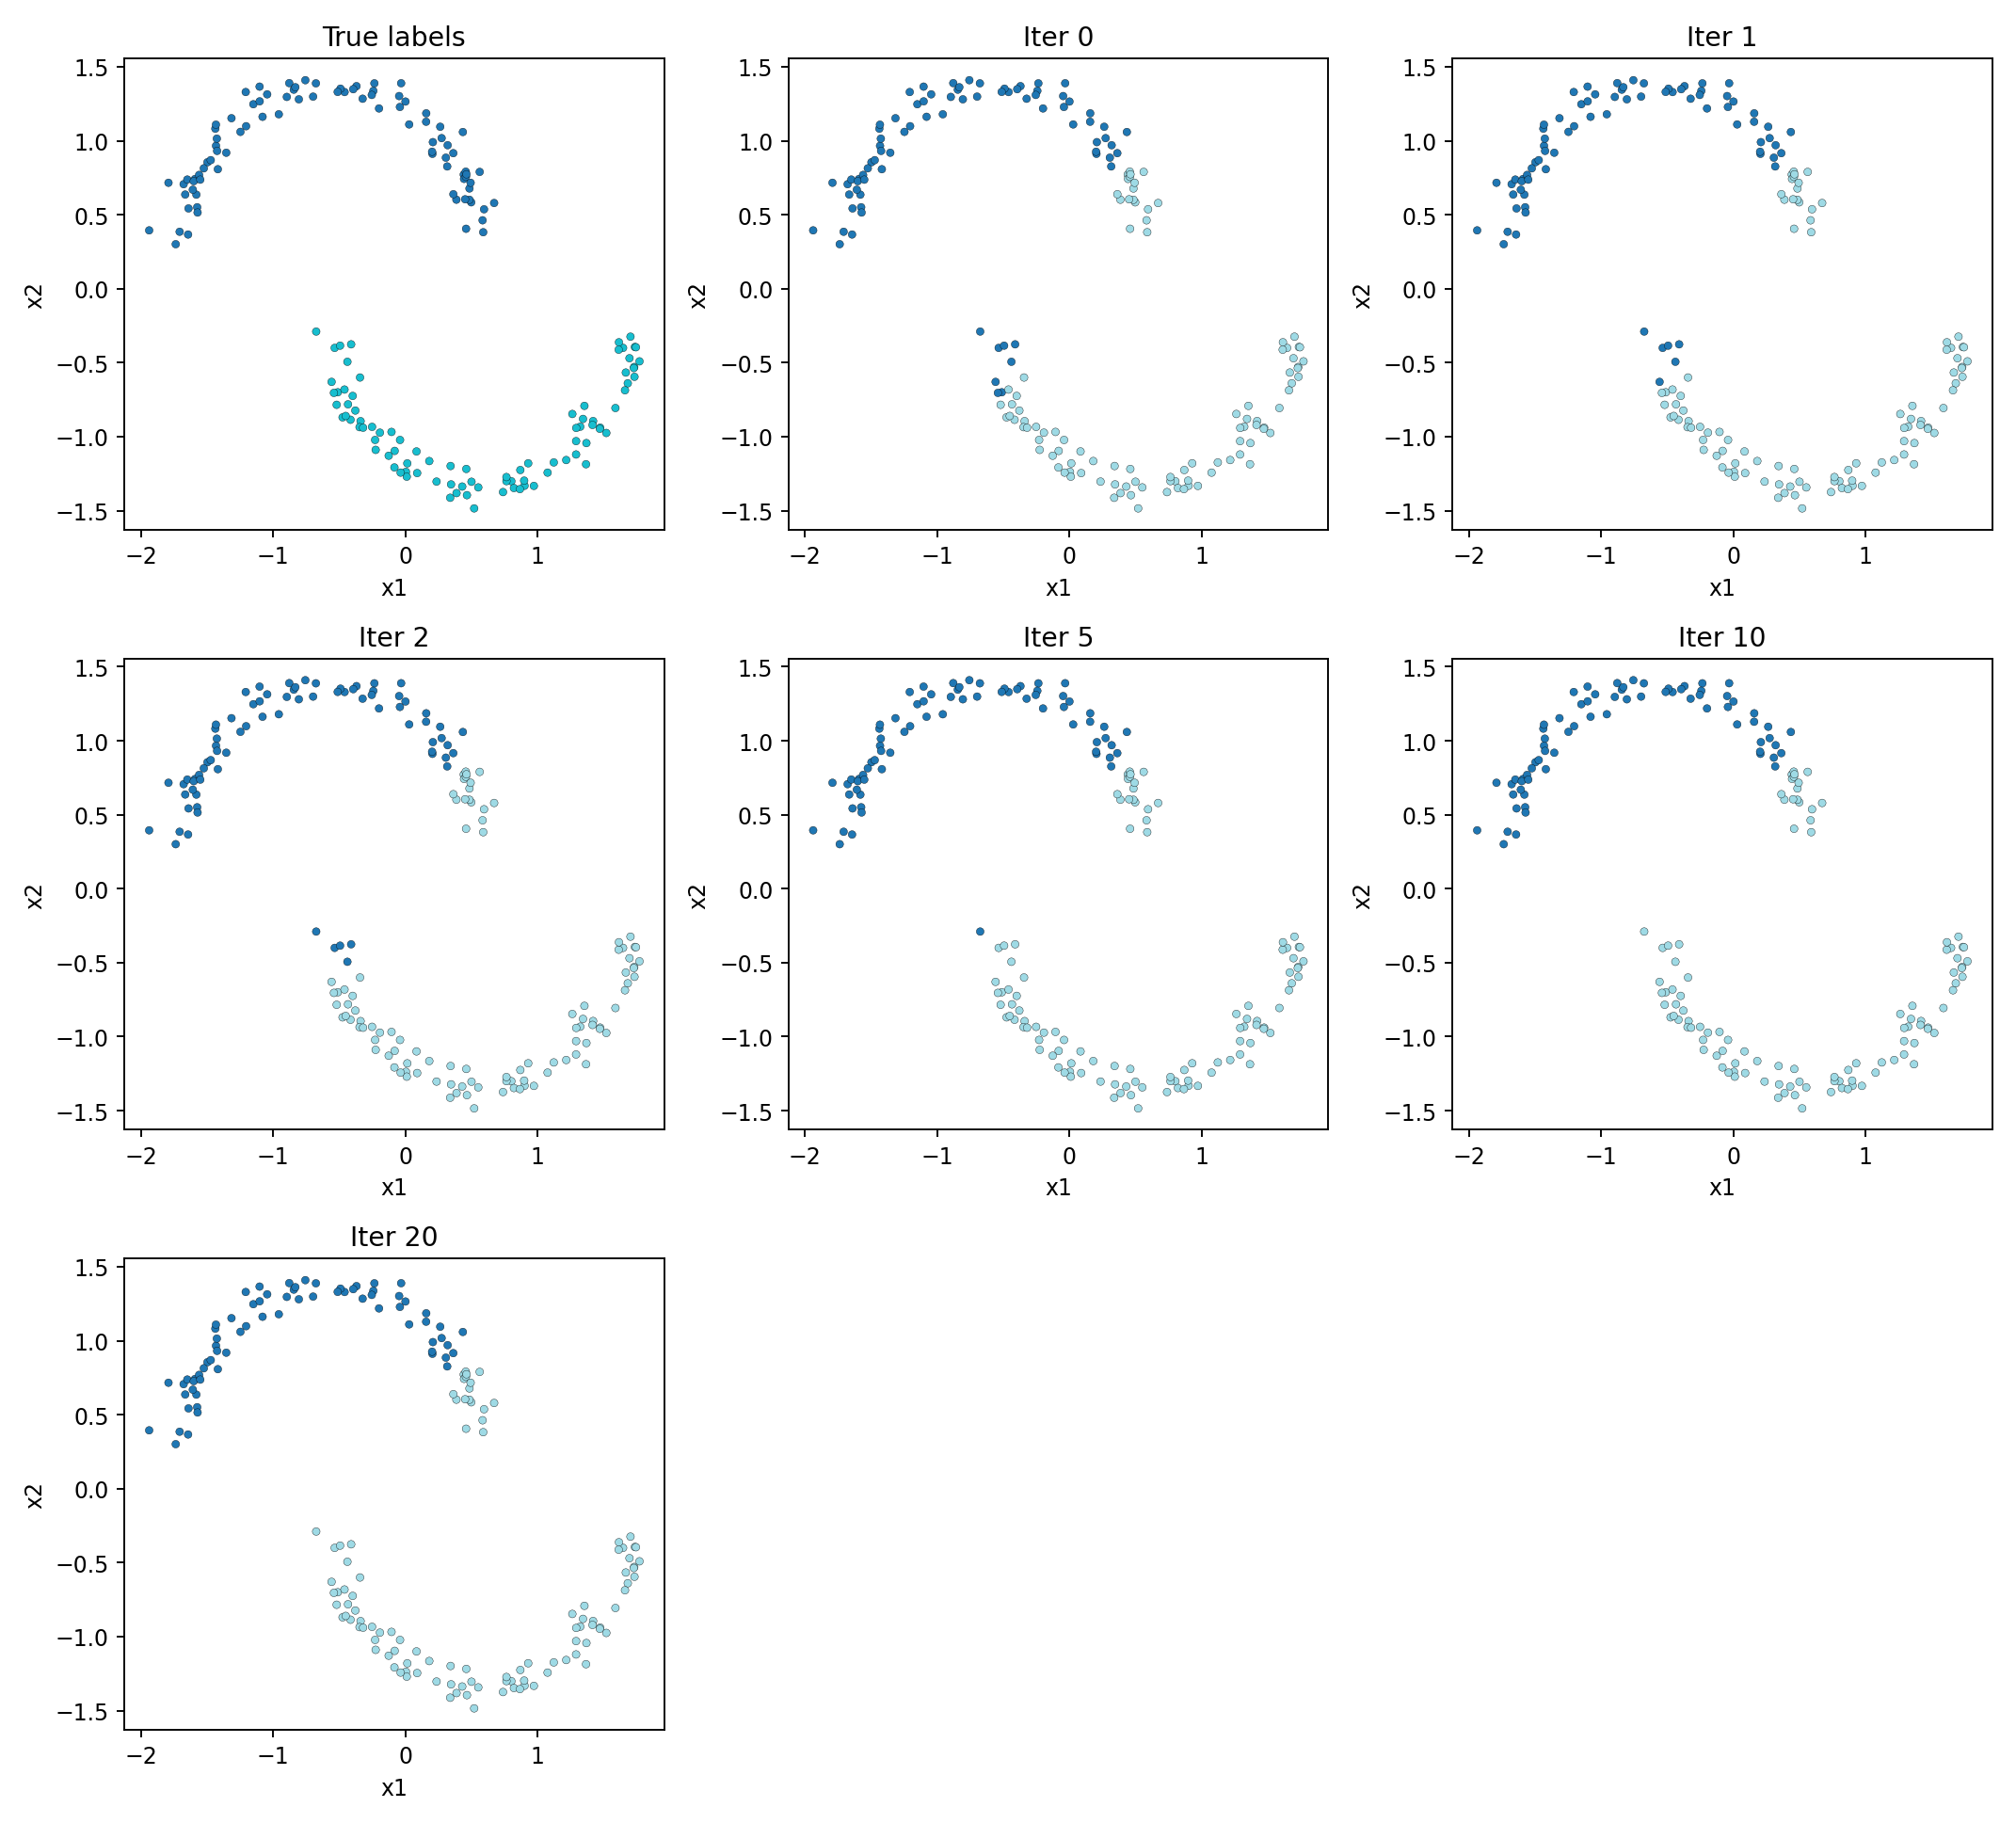
\includegraphics[width=\linewidth]{figs/synth_stage_04_iter_snapshots.png}
  \caption{Moons (iters)}
\end{subfigure}
\begin{subfigure}{0.48\linewidth}
  \centering
  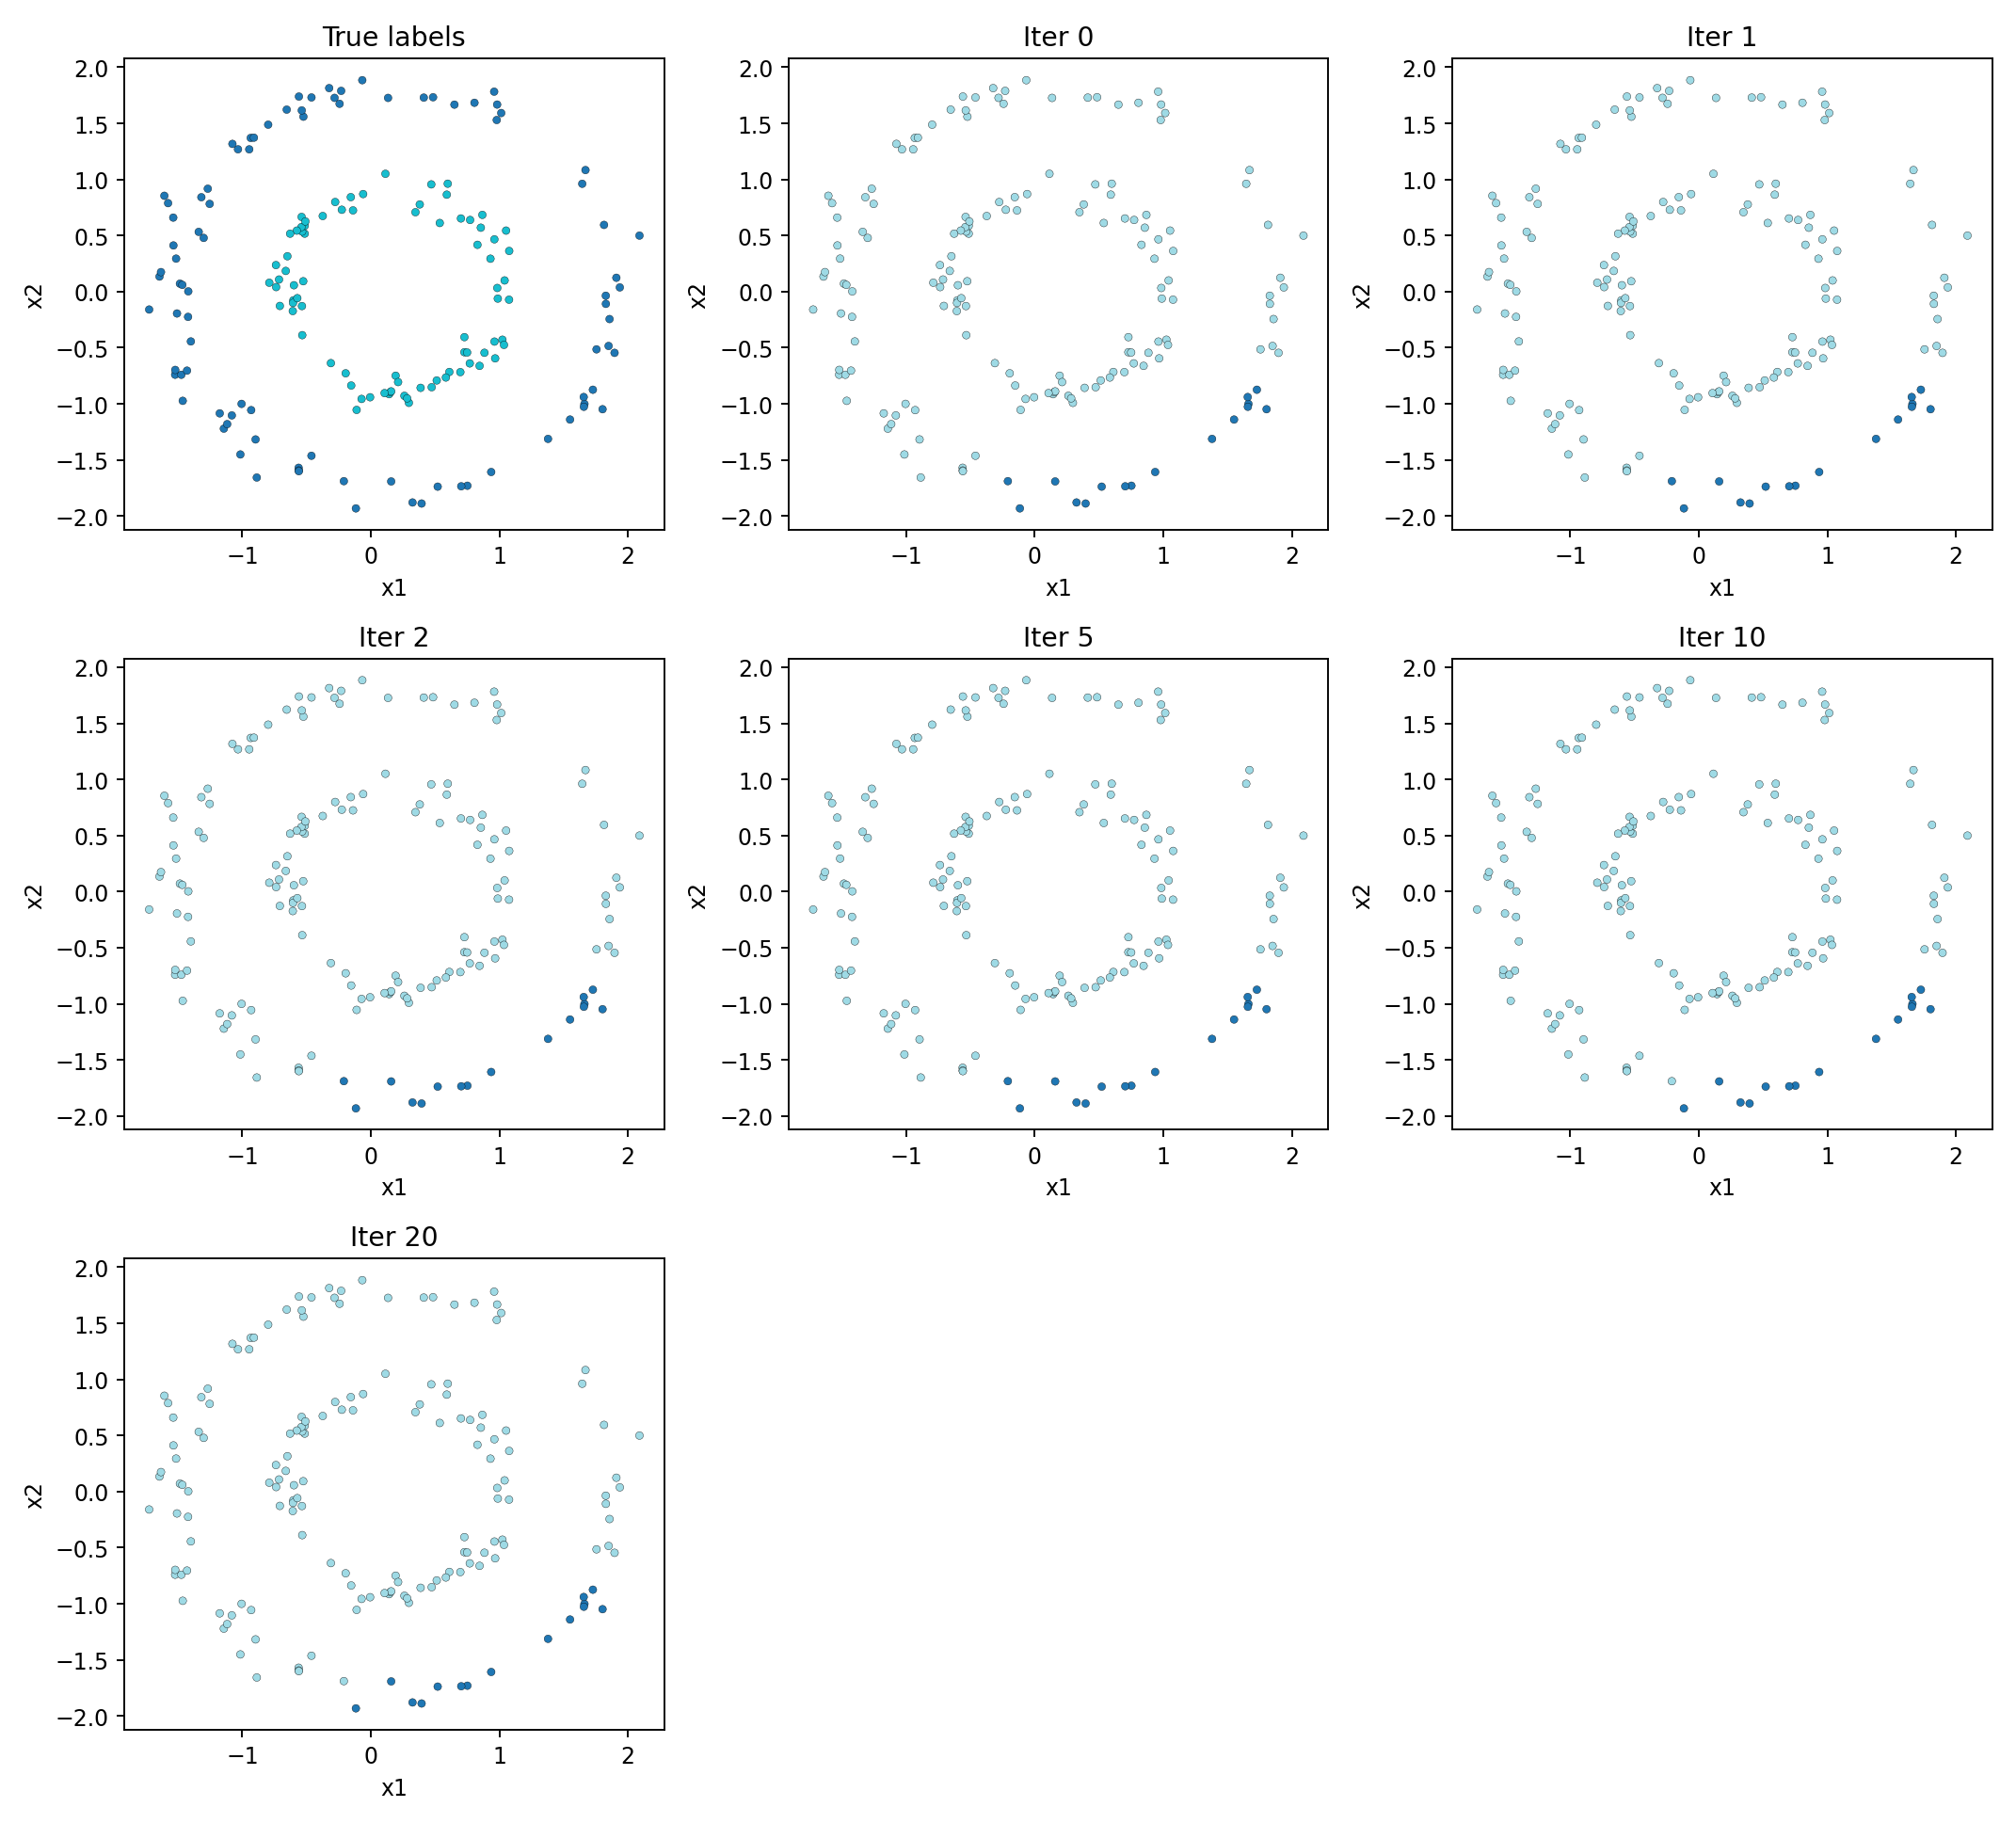
\includegraphics[width=\linewidth]{figs/synth_circles_iter.png}
  \caption{Circles (iters)}
\end{subfigure}
\begin{subfigure}{0.48\linewidth}
  \centering
  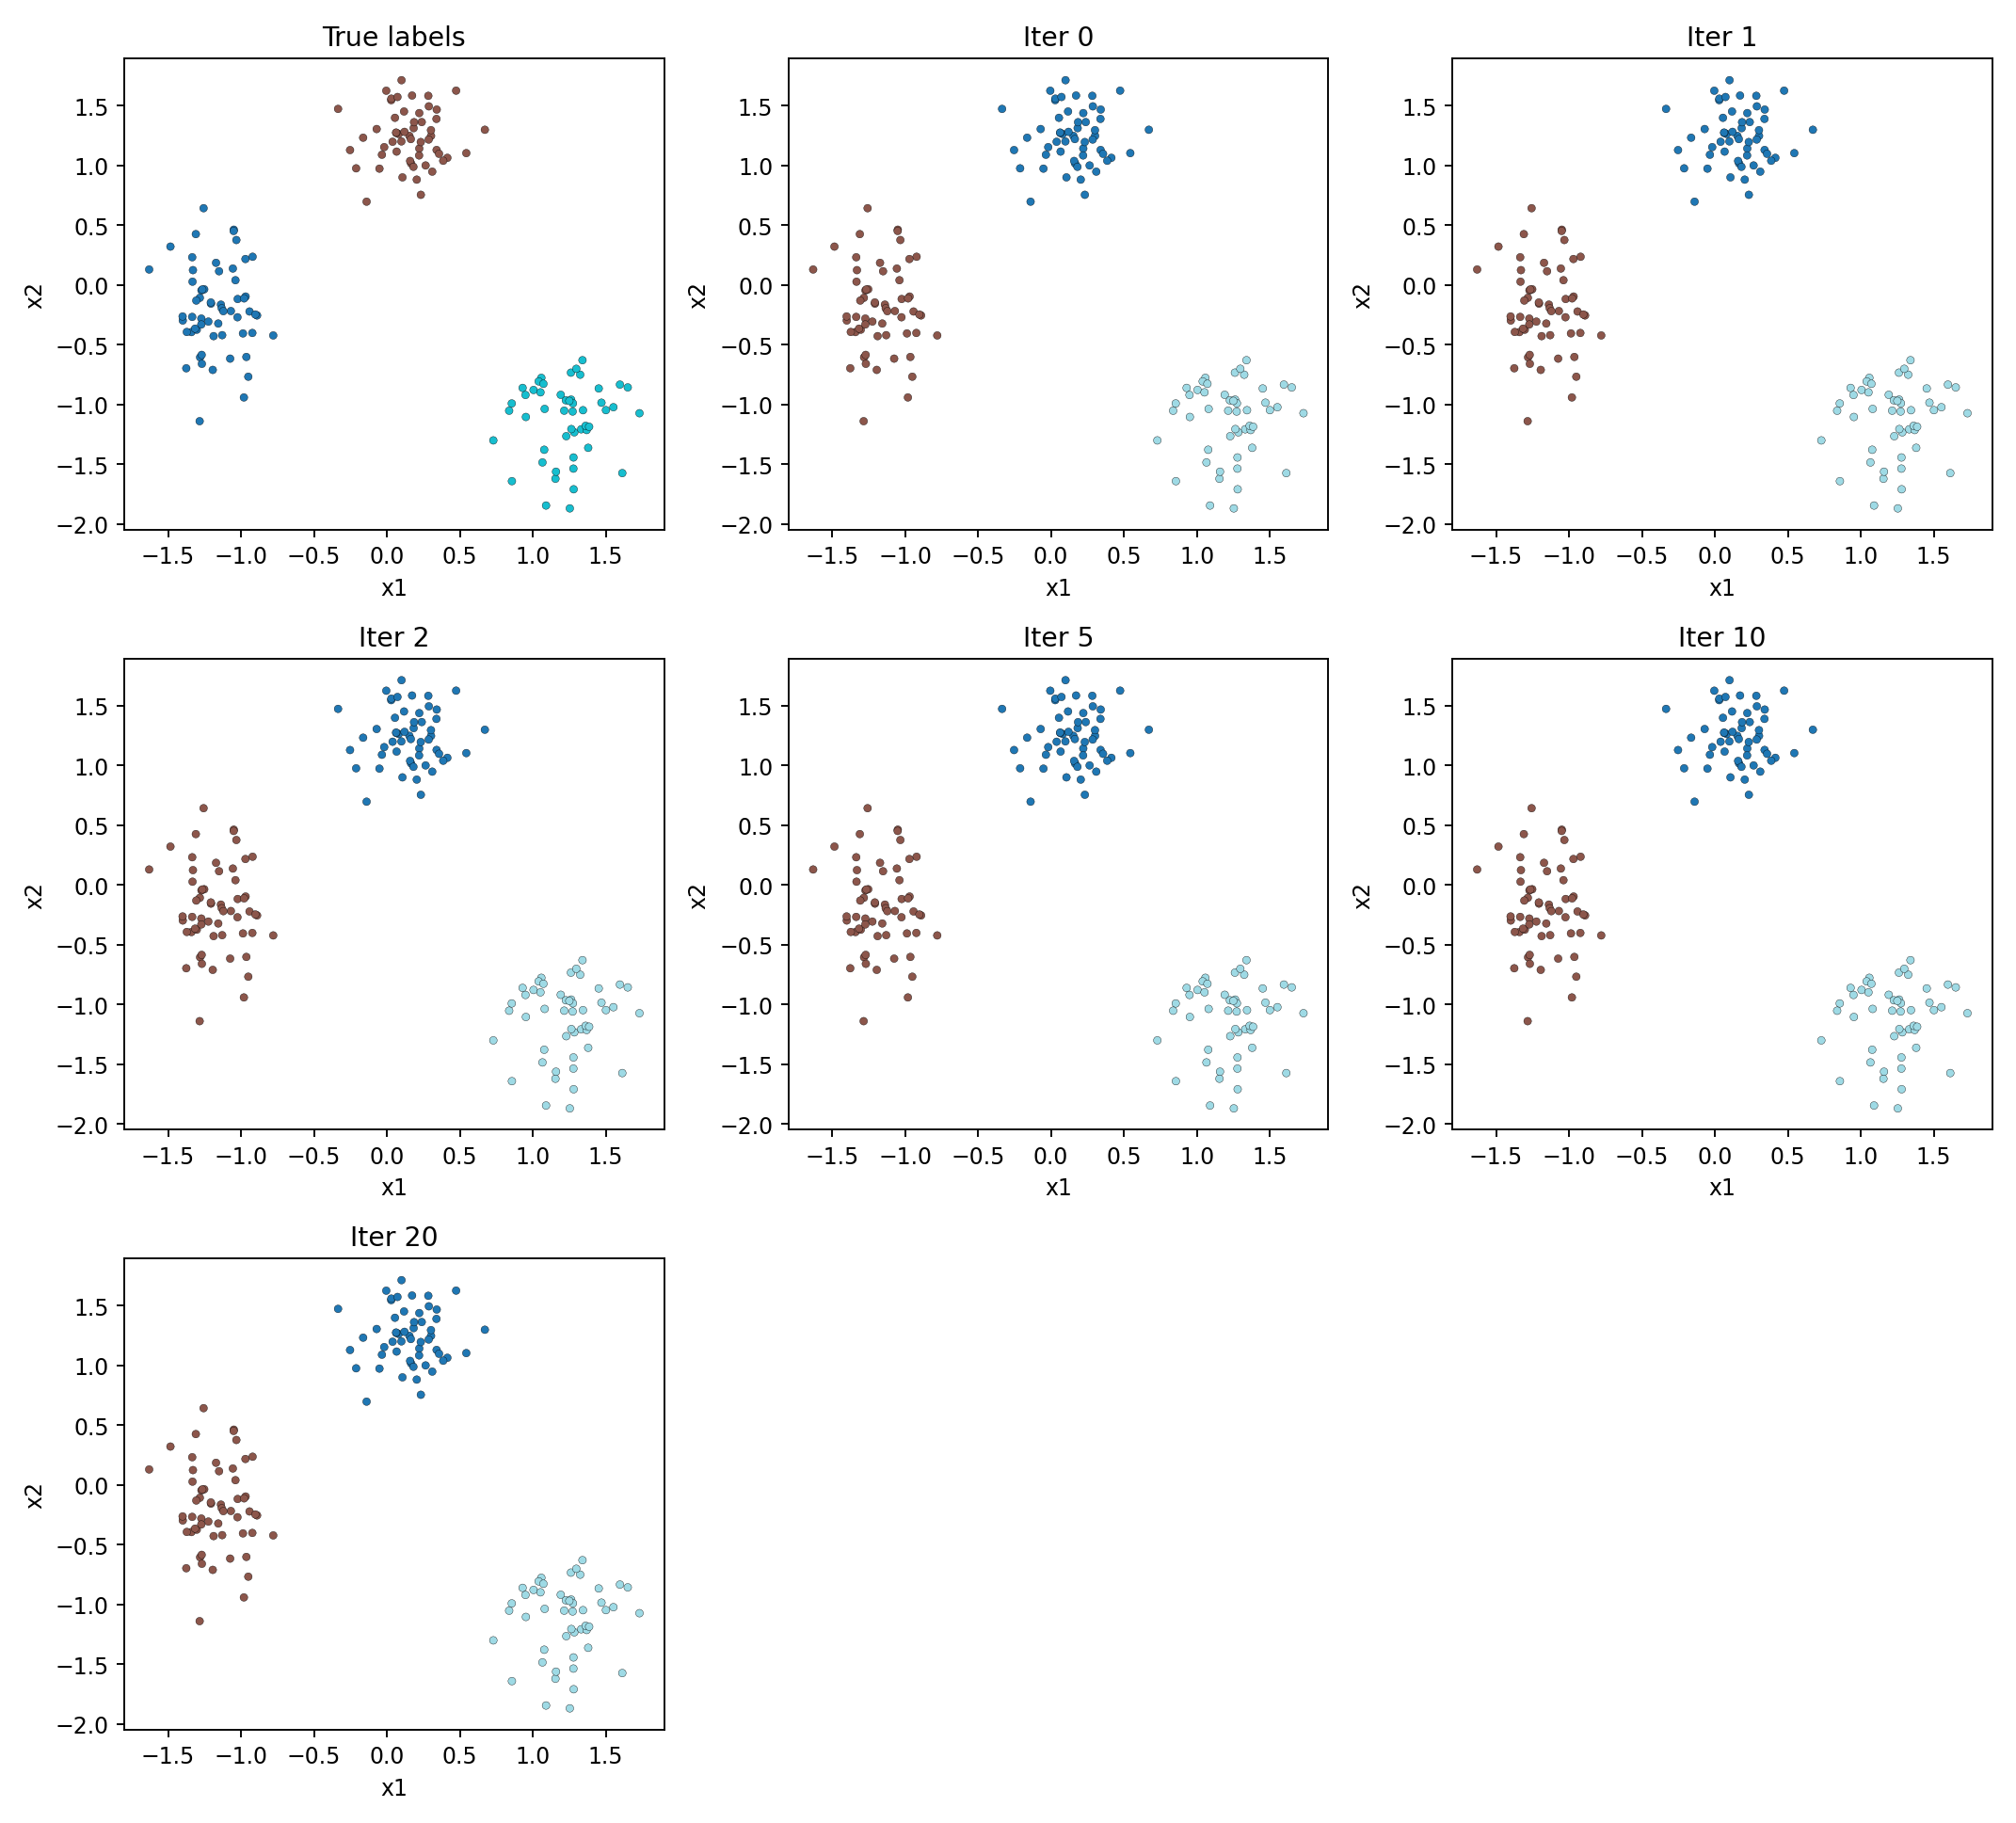
\includegraphics[width=\linewidth]{figs/synth_gaussians_iter.png}
  \caption{Gaussians (iters)}
\end{subfigure}
\begin{subfigure}{0.48\linewidth}
  \centering
  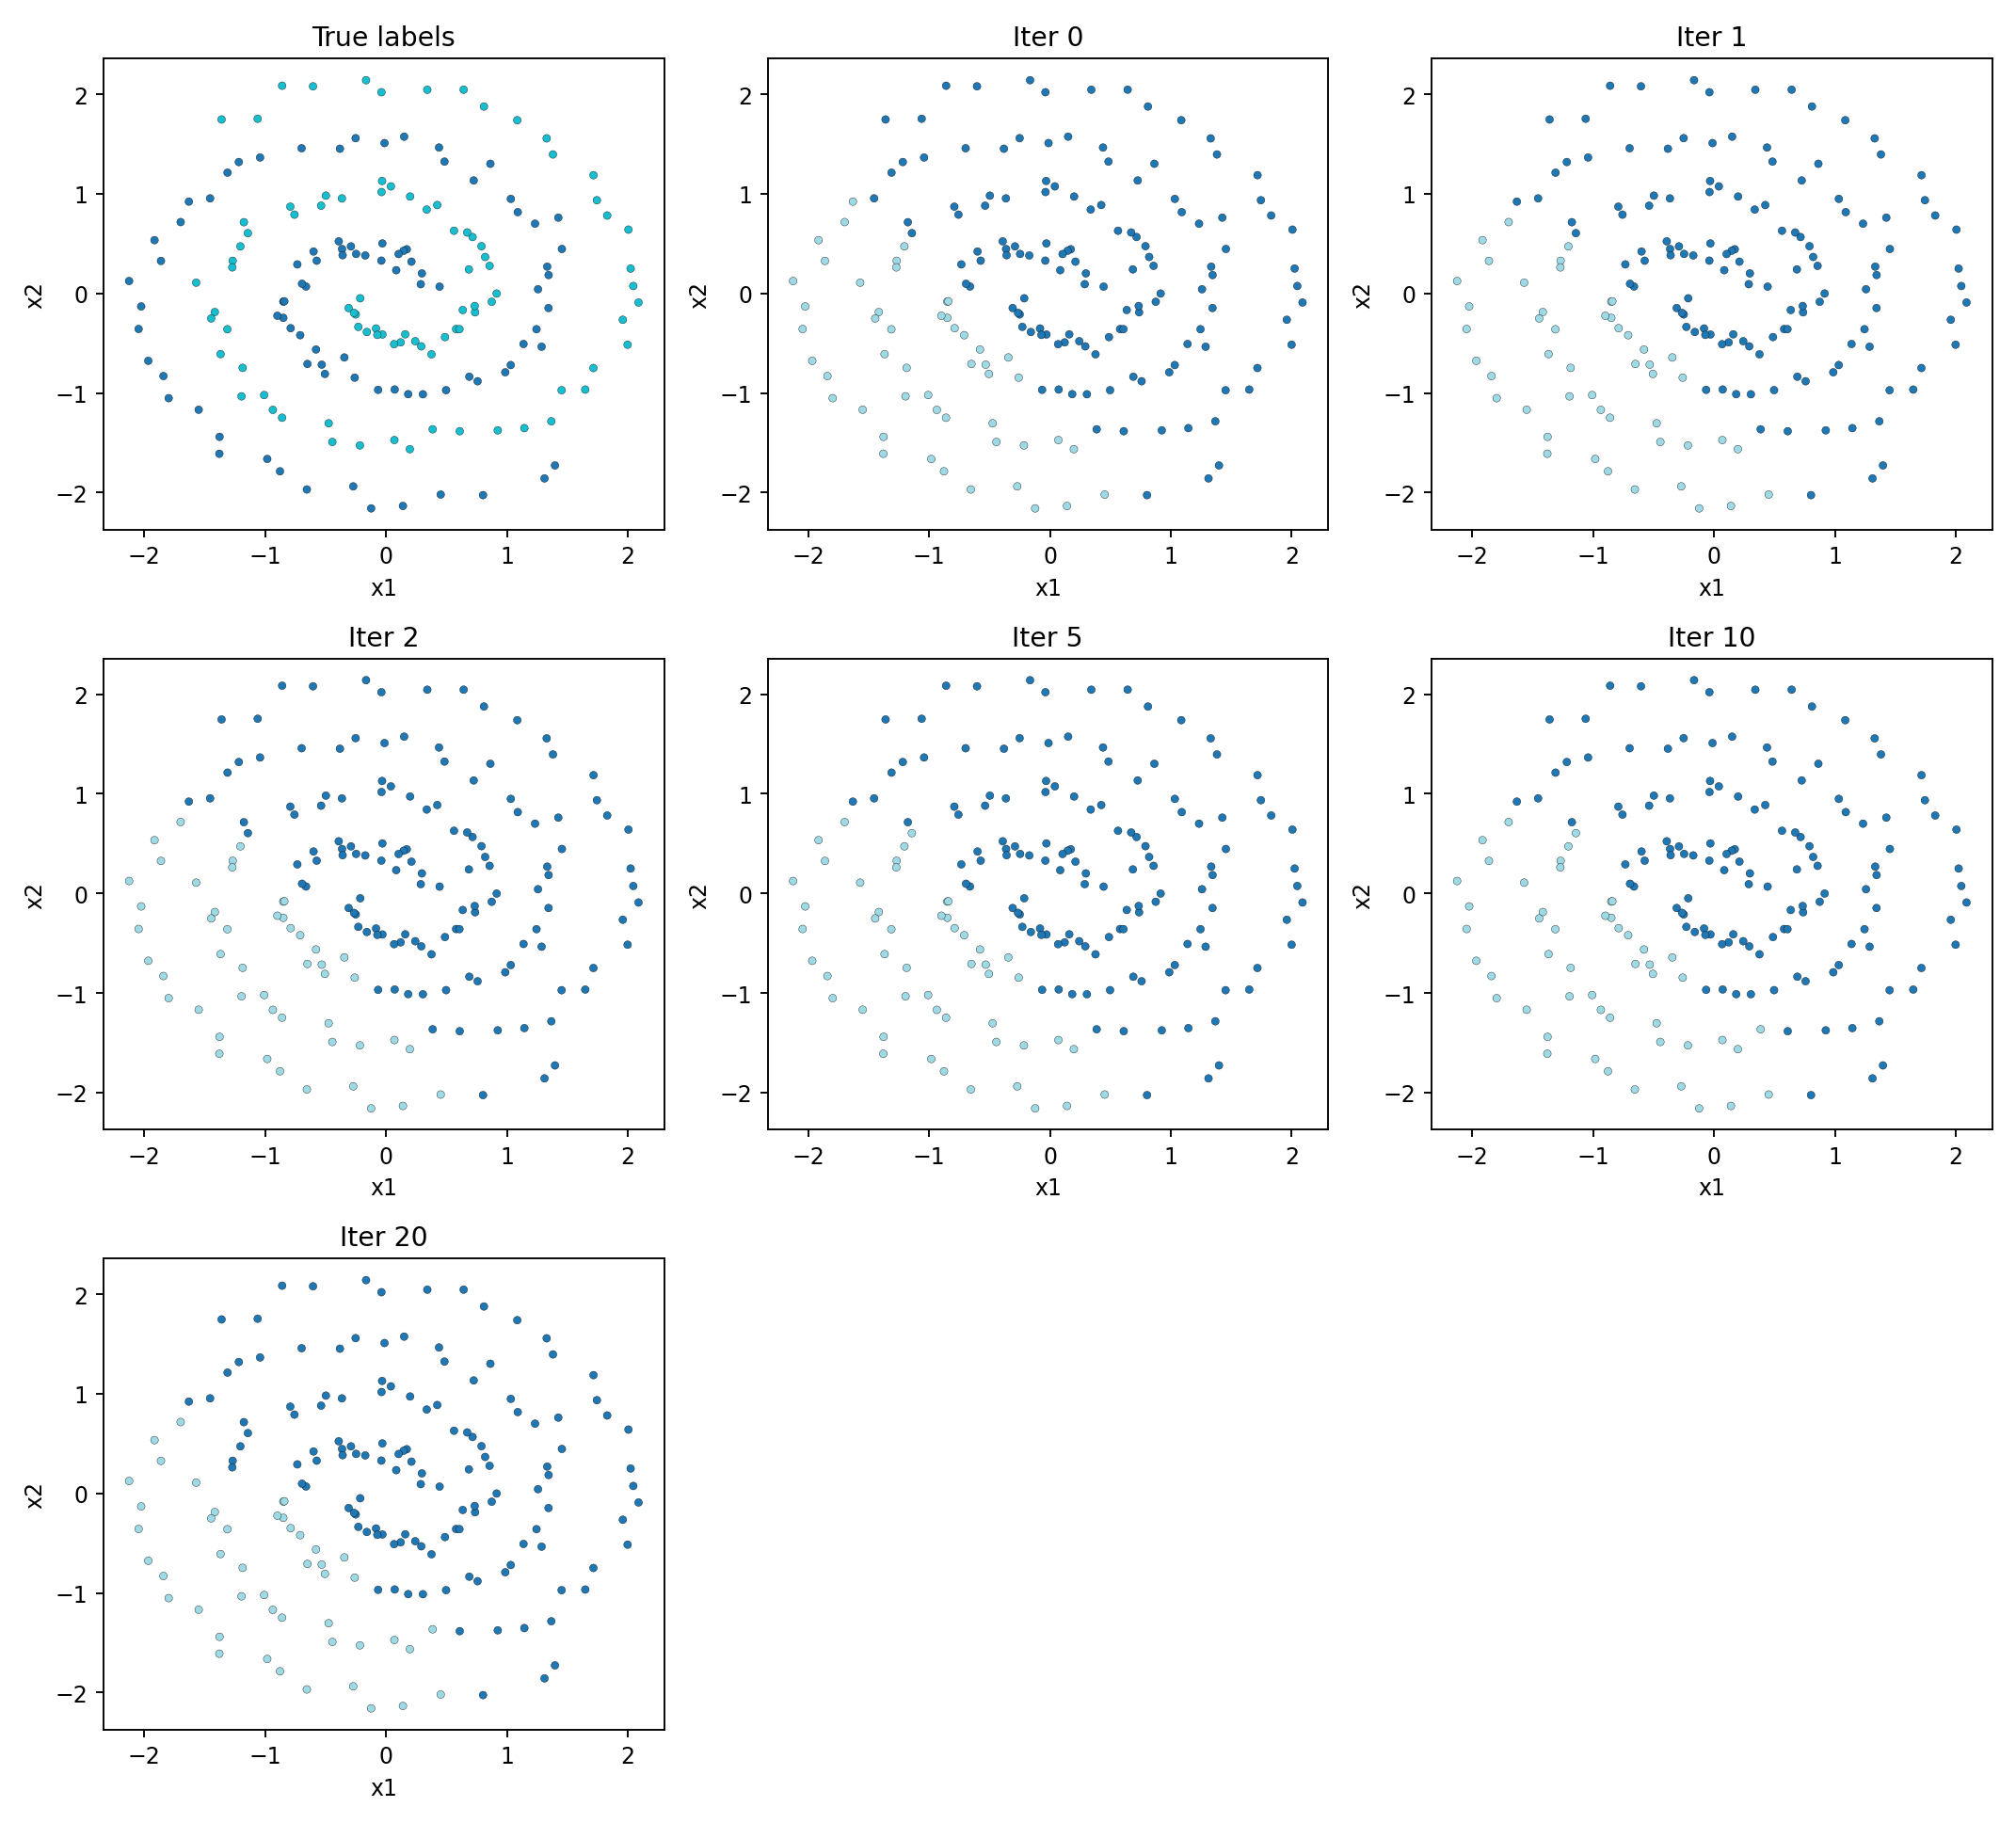
\includegraphics[width=\linewidth]{figs/synth_spiral_iter.png}
  \caption{Spiral (iters)}
\end{subfigure}
\caption{Synthetic datasets and torque clustering iteration snapshots.}
\label{fig:synthetic}
\end{figure}

\begin{figure}[t]
\centering
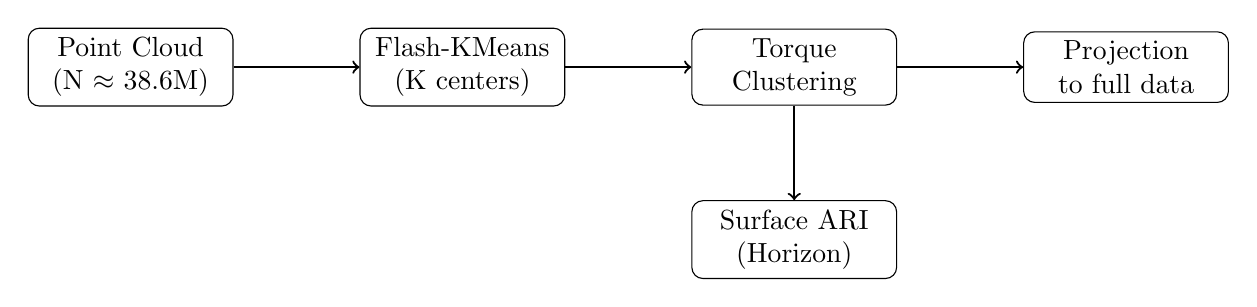
\begin{tikzpicture}[
    box/.style={draw, rounded corners, minimum height=0.8cm, minimum width=2.6cm, align=center},
    arrow/.style={->, thick}
]
\node[box] (data) {Point Cloud\\(N $\approx$ 38.6M)};
\node[box, right=1.6cm of data] (kmeans) {Flash-KMeans\\(K centers)};
\node[box, right=1.6cm of kmeans] (torque) {Torque\\Clustering};
\node[box, right=1.6cm of torque] (proj) {Projection\\to full data};
\node[box, below=1.2cm of torque] (surface) {Surface ARI\\(Horizon)};

\draw[arrow] (data) -- (kmeans);
\draw[arrow] (kmeans) -- (torque);
\draw[arrow] (torque) -- (proj);
\draw[arrow] (torque) -- (surface);
\end{tikzpicture}

\caption{Pipeline overview: Flash-KMeans $\rightarrow$ Torque $\rightarrow$ Projection.}
\label{fig:pipeline}
\end{figure}

\subsection{Real Seismic Data}
\begin{figure}[t]
\centering
\begin{subfigure}{0.48\linewidth}
  \centering
  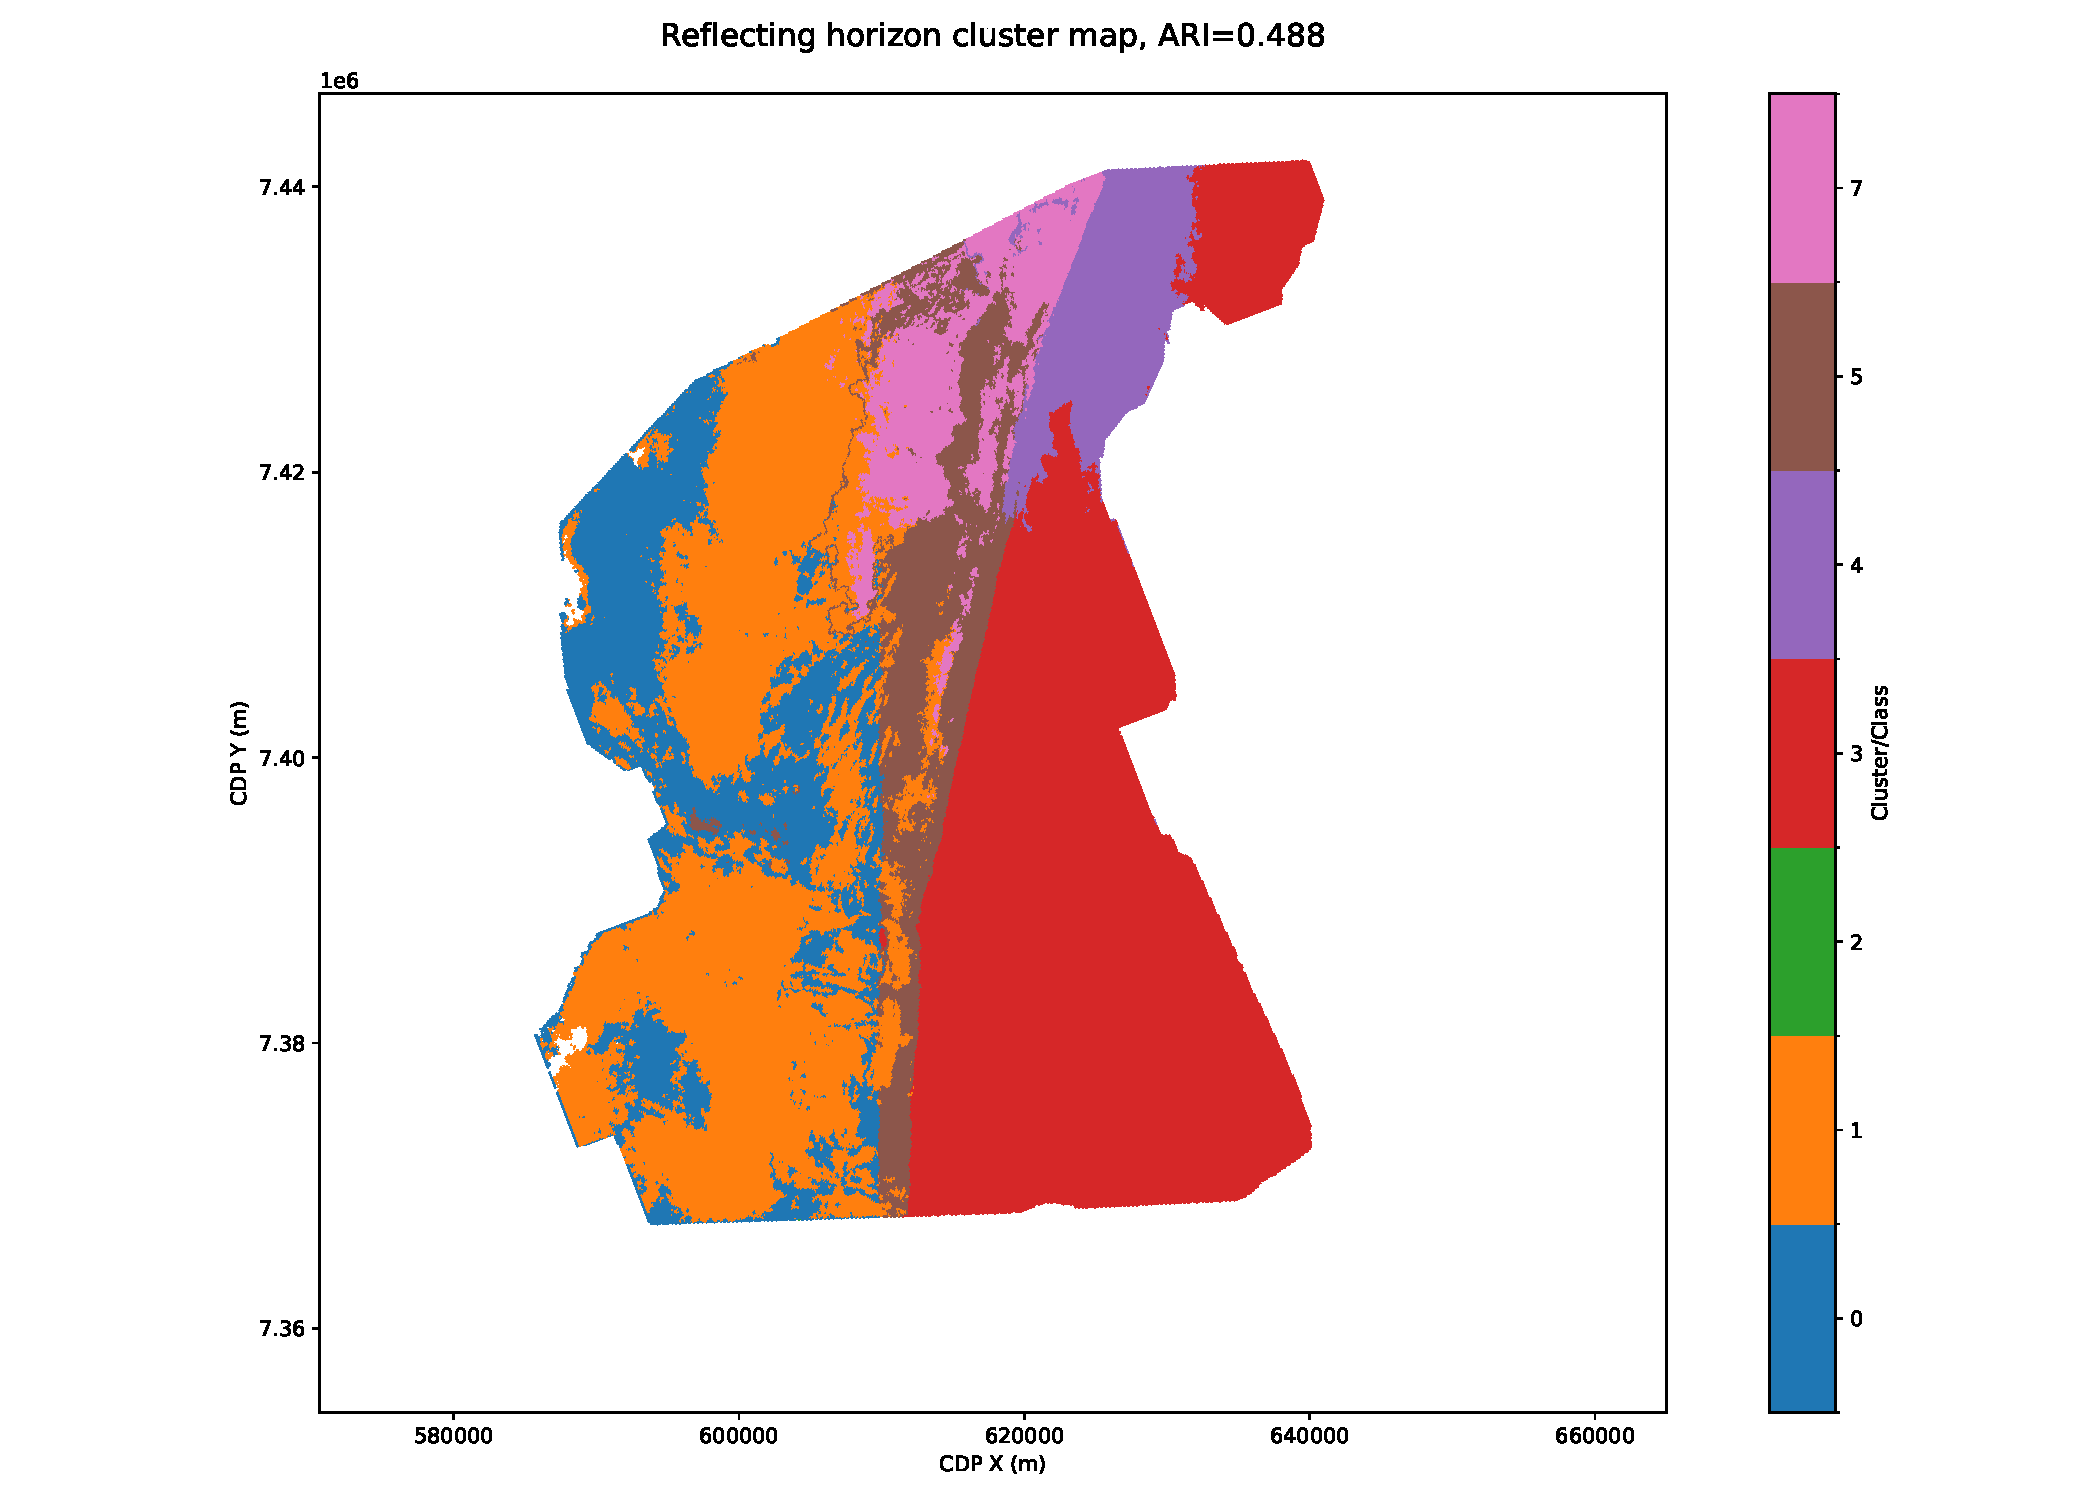
\includegraphics[width=\linewidth]{figs/iter_000_surface_ari_map.pdf}
  \caption{Iter 0}
\end{subfigure}
\begin{subfigure}{0.48\linewidth}
  \centering
  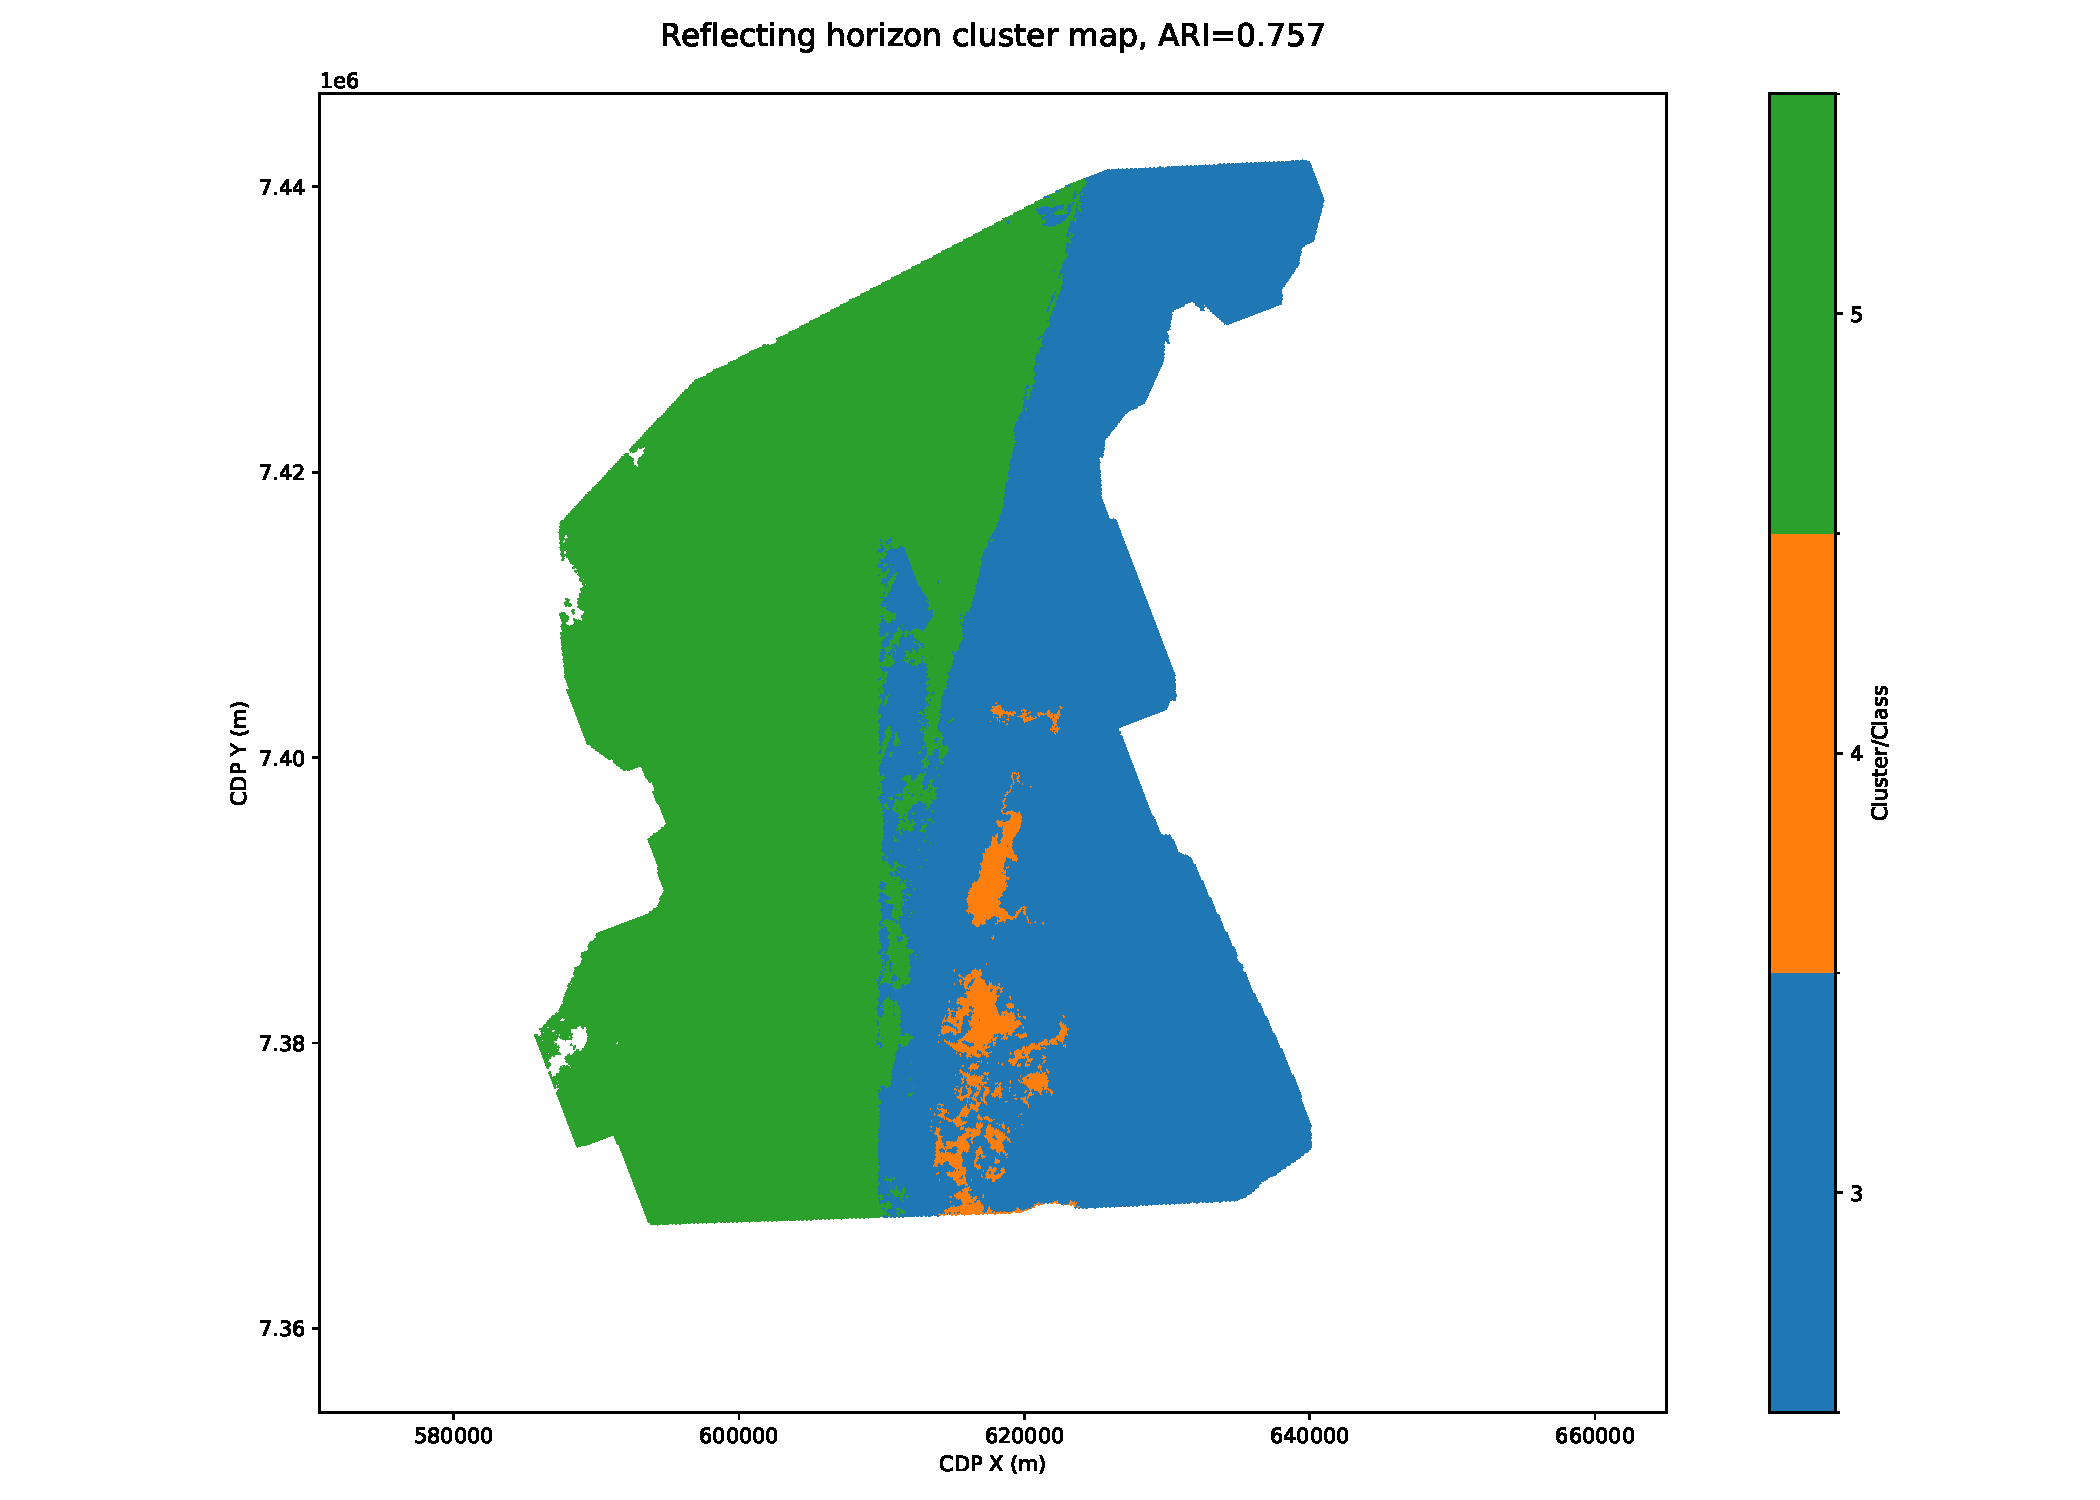
\includegraphics[width=\linewidth]{figs/iter_002_surface_ari_map.pdf}
  \caption{Iter 2}
\end{subfigure}
\begin{subfigure}{0.48\linewidth}
  \centering
  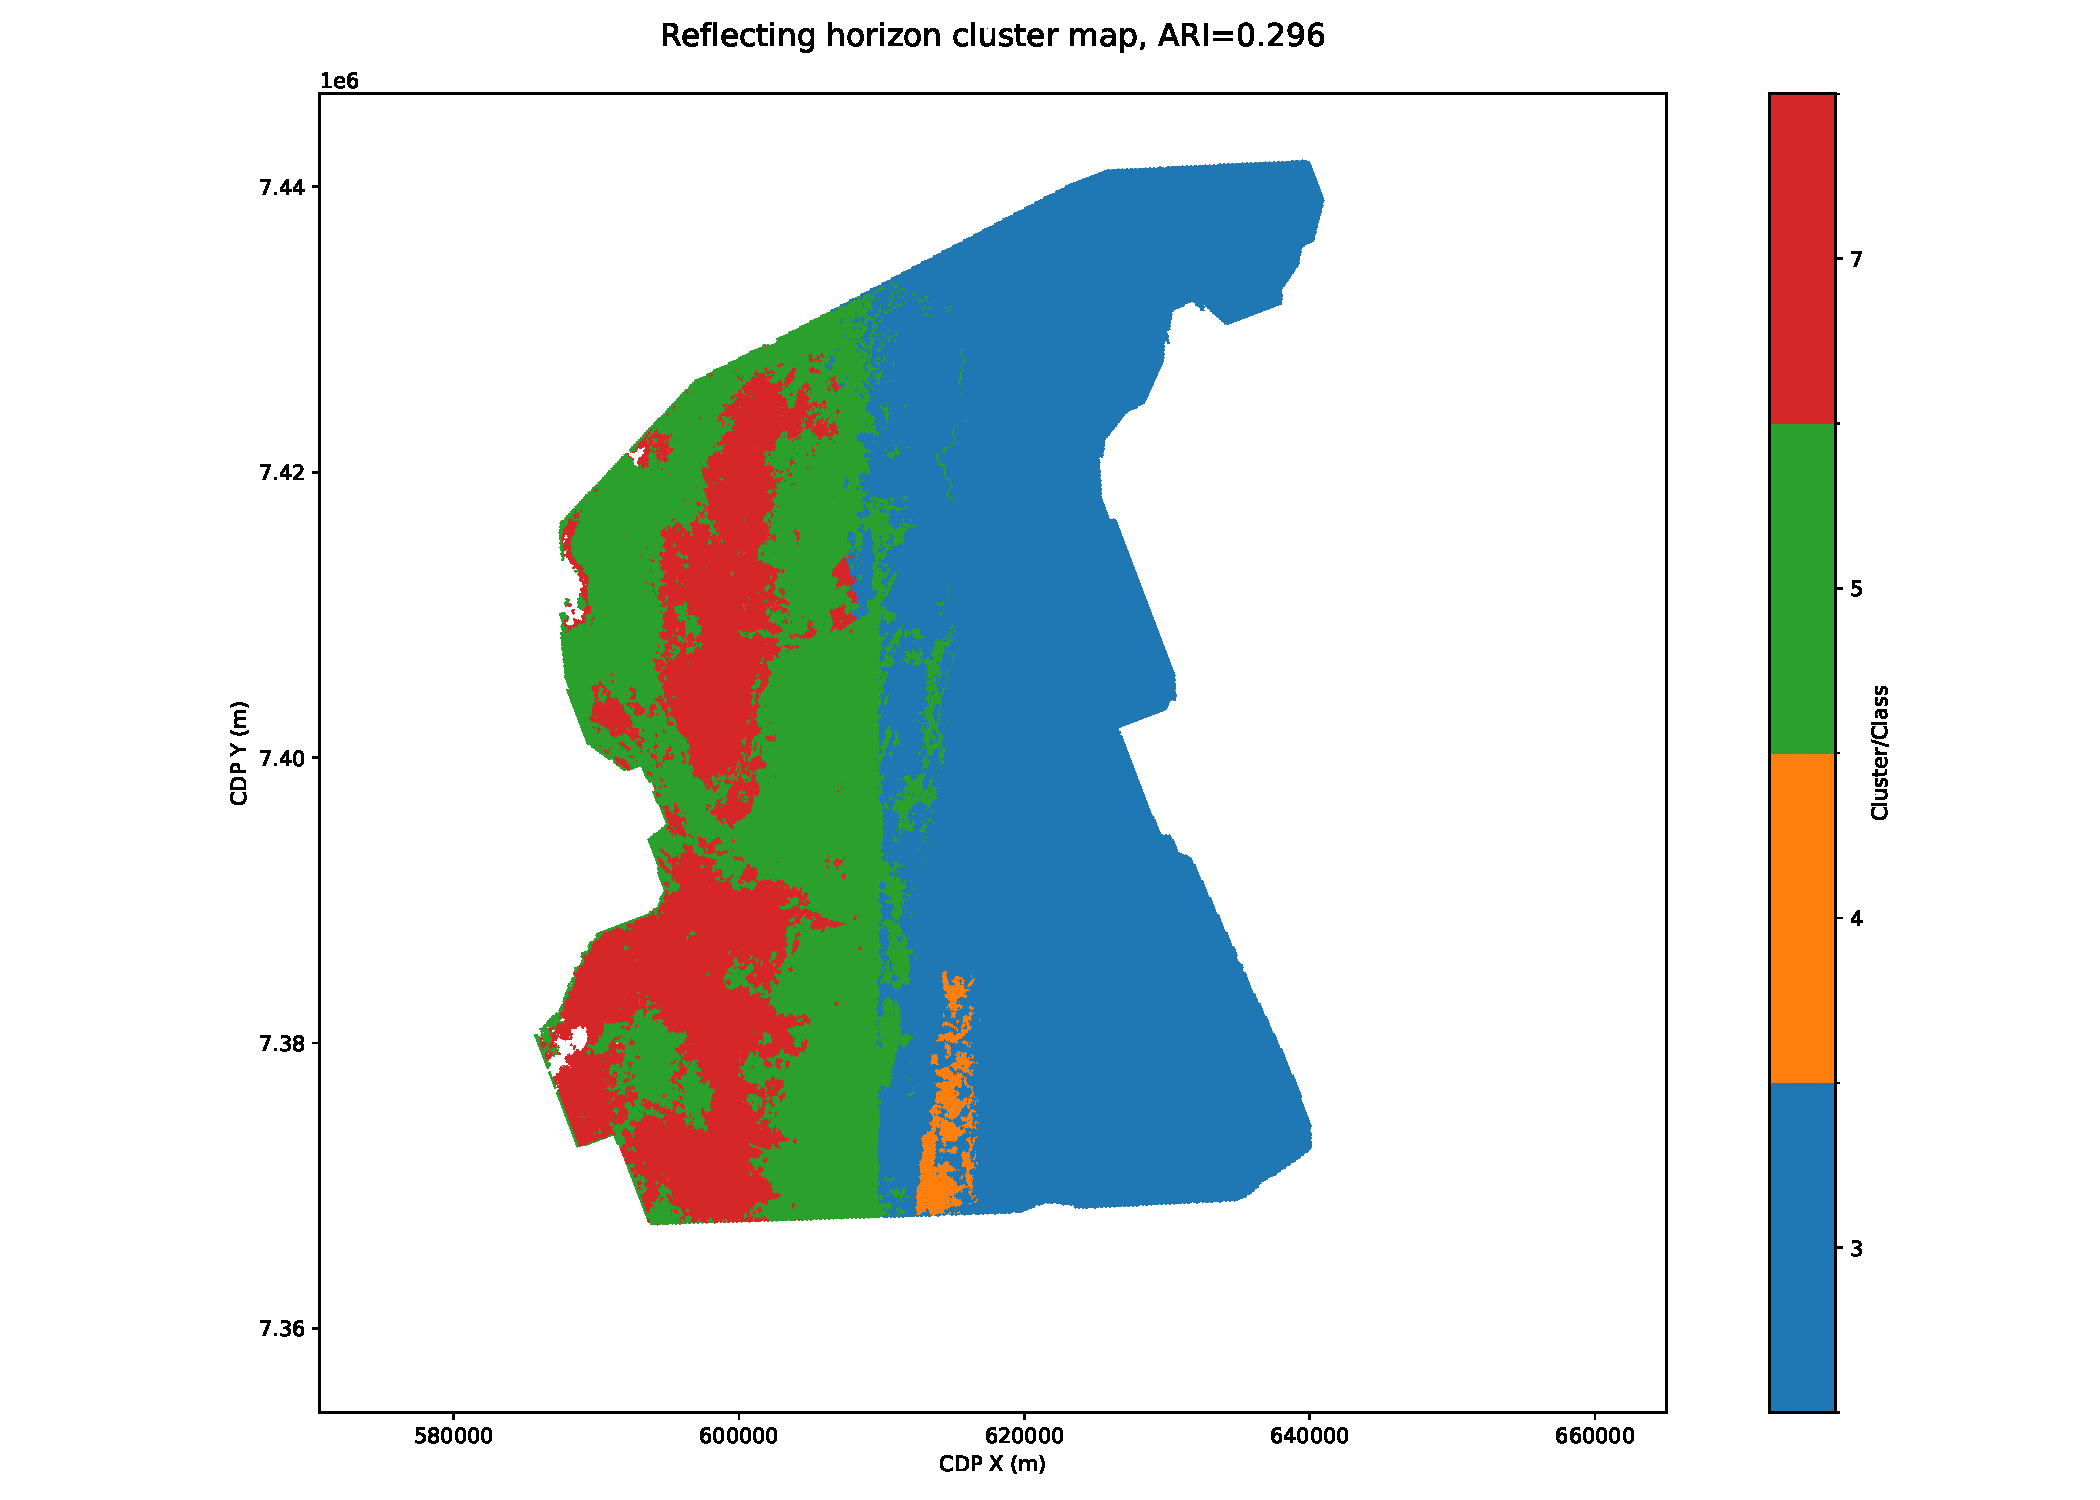
\includegraphics[width=\linewidth]{figs/iter_004_surface_ari_map.pdf}
  \caption{Iter 4}
\end{subfigure}
\begin{subfigure}{0.48\linewidth}
  \centering
  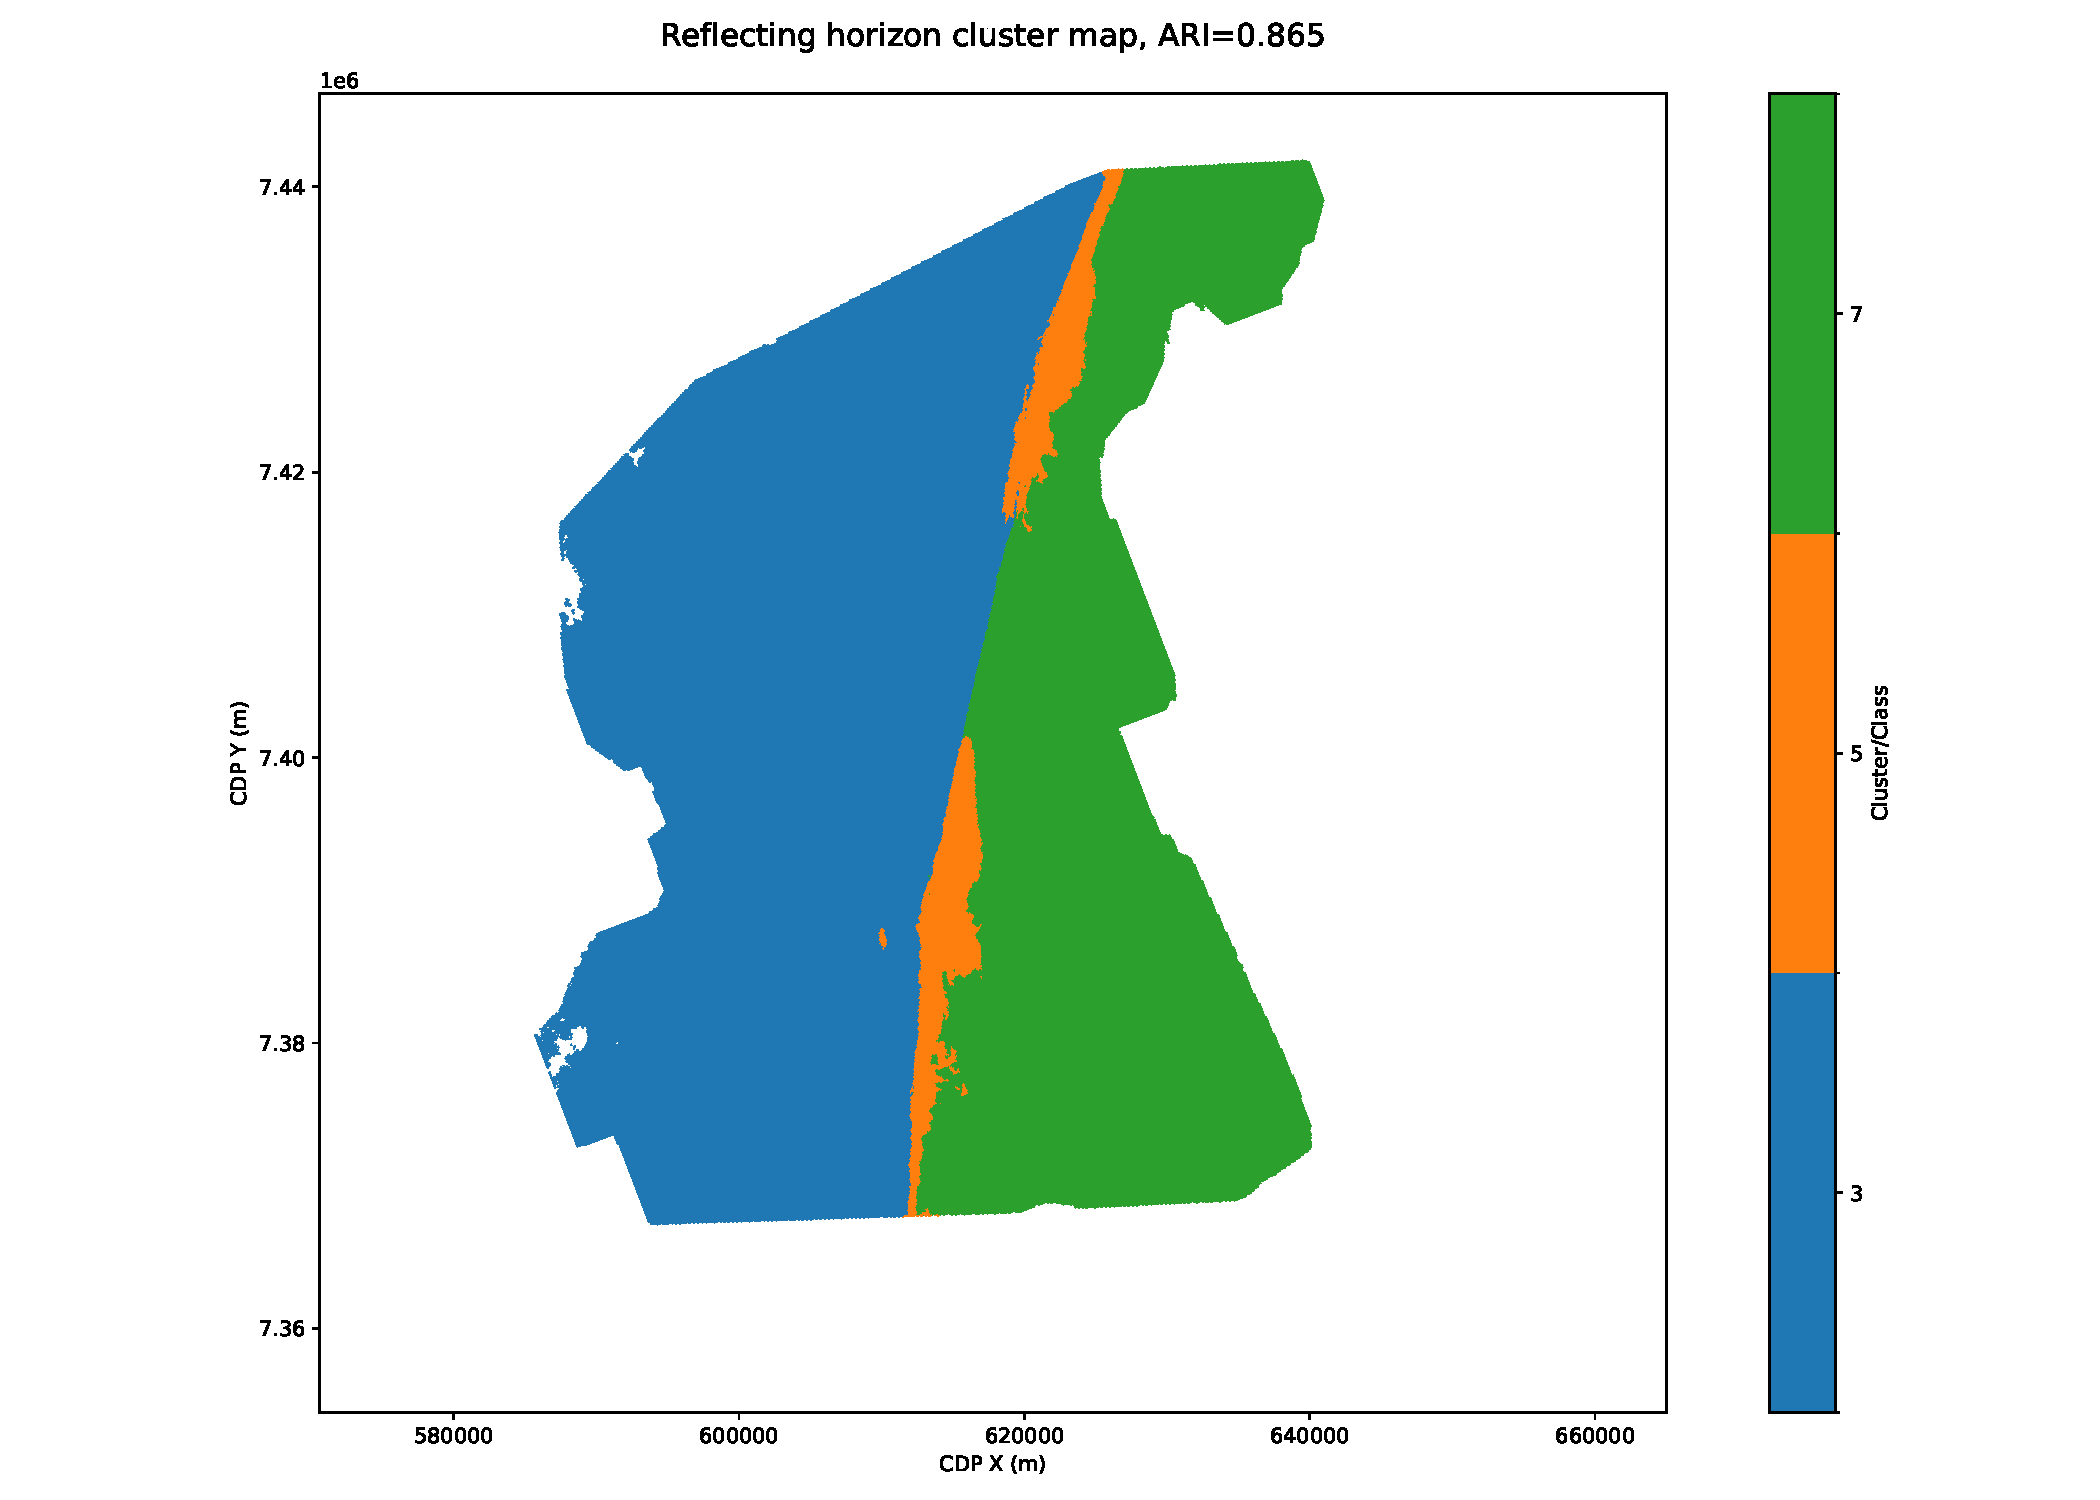
\includegraphics[width=\linewidth]{figs/iter_006_surface_ari_map.pdf}
  \caption{Iter 6 (best)}
\end{subfigure}
\caption{Surface-projected clustering across ADMM iterations.}
\label{fig:iters}
\end{figure}

\begin{figure}[t]
\centering
\includegraphics[width=0.95\linewidth]{figs/final_surface_ari_map.pdf}
\caption{Final surface-projected clustering (best run).}
\label{fig:final_surface}
\end{figure}

\begin{figure}[t]
\centering
\begin{subfigure}{0.48\linewidth}
  \centering
  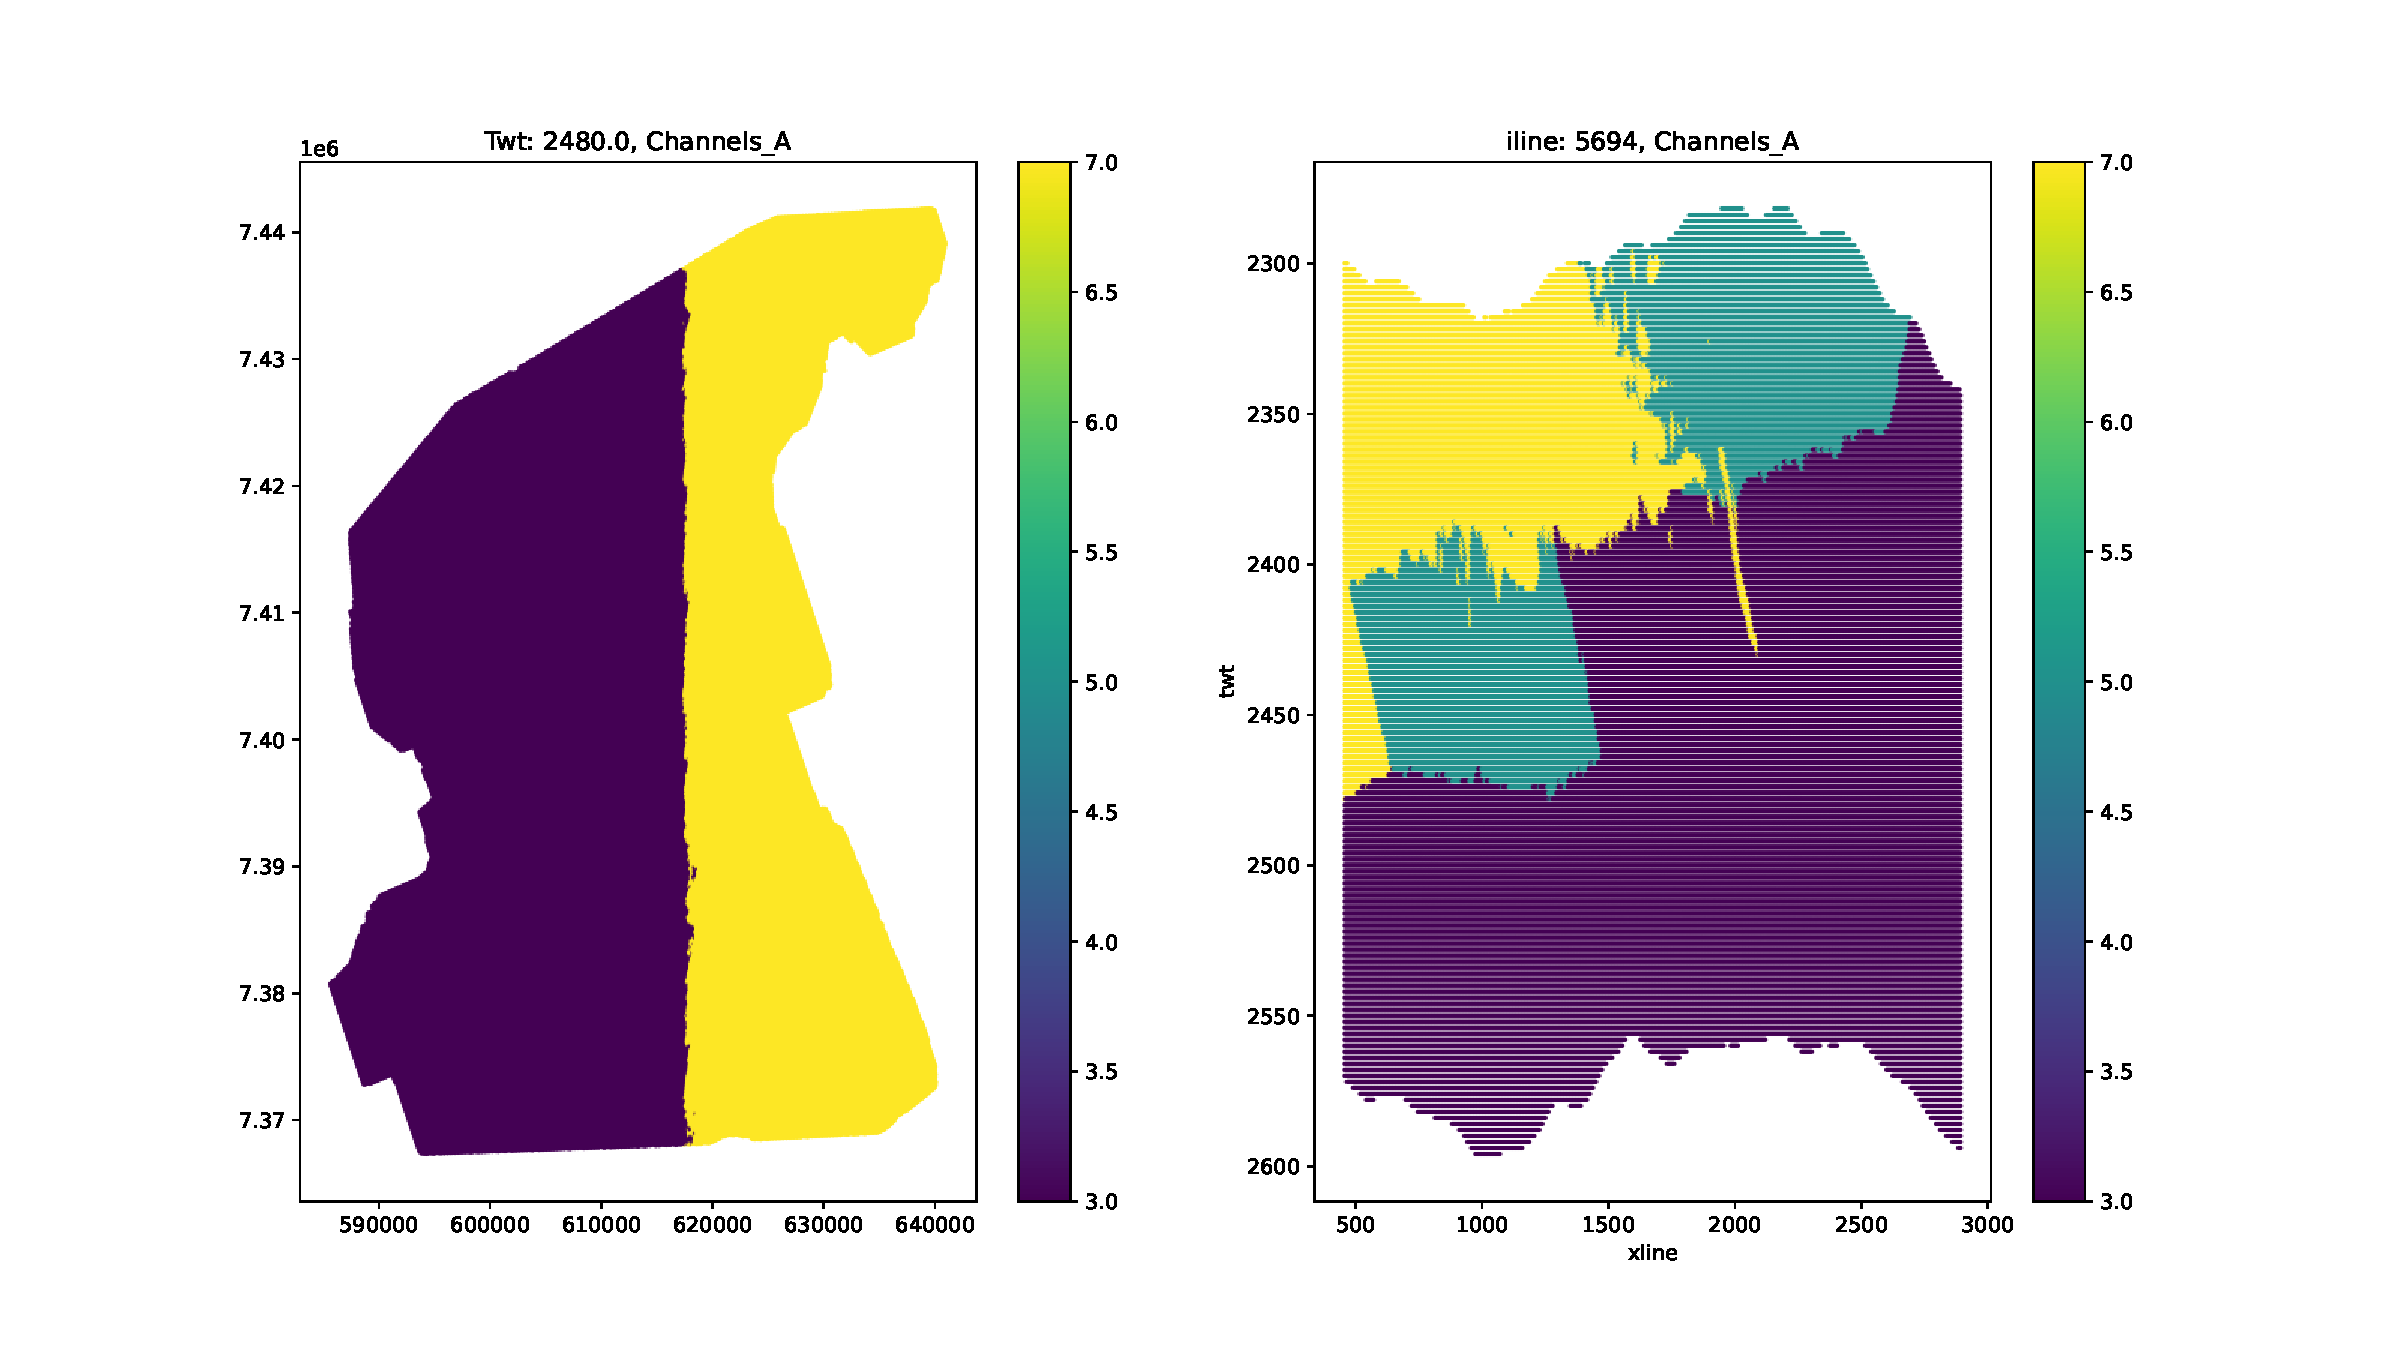
\includegraphics[width=\linewidth]{figs/cross_channels_iter6.pdf}
  \caption{Channels}
\end{subfigure}
\begin{subfigure}{0.48\linewidth}
  \centering
  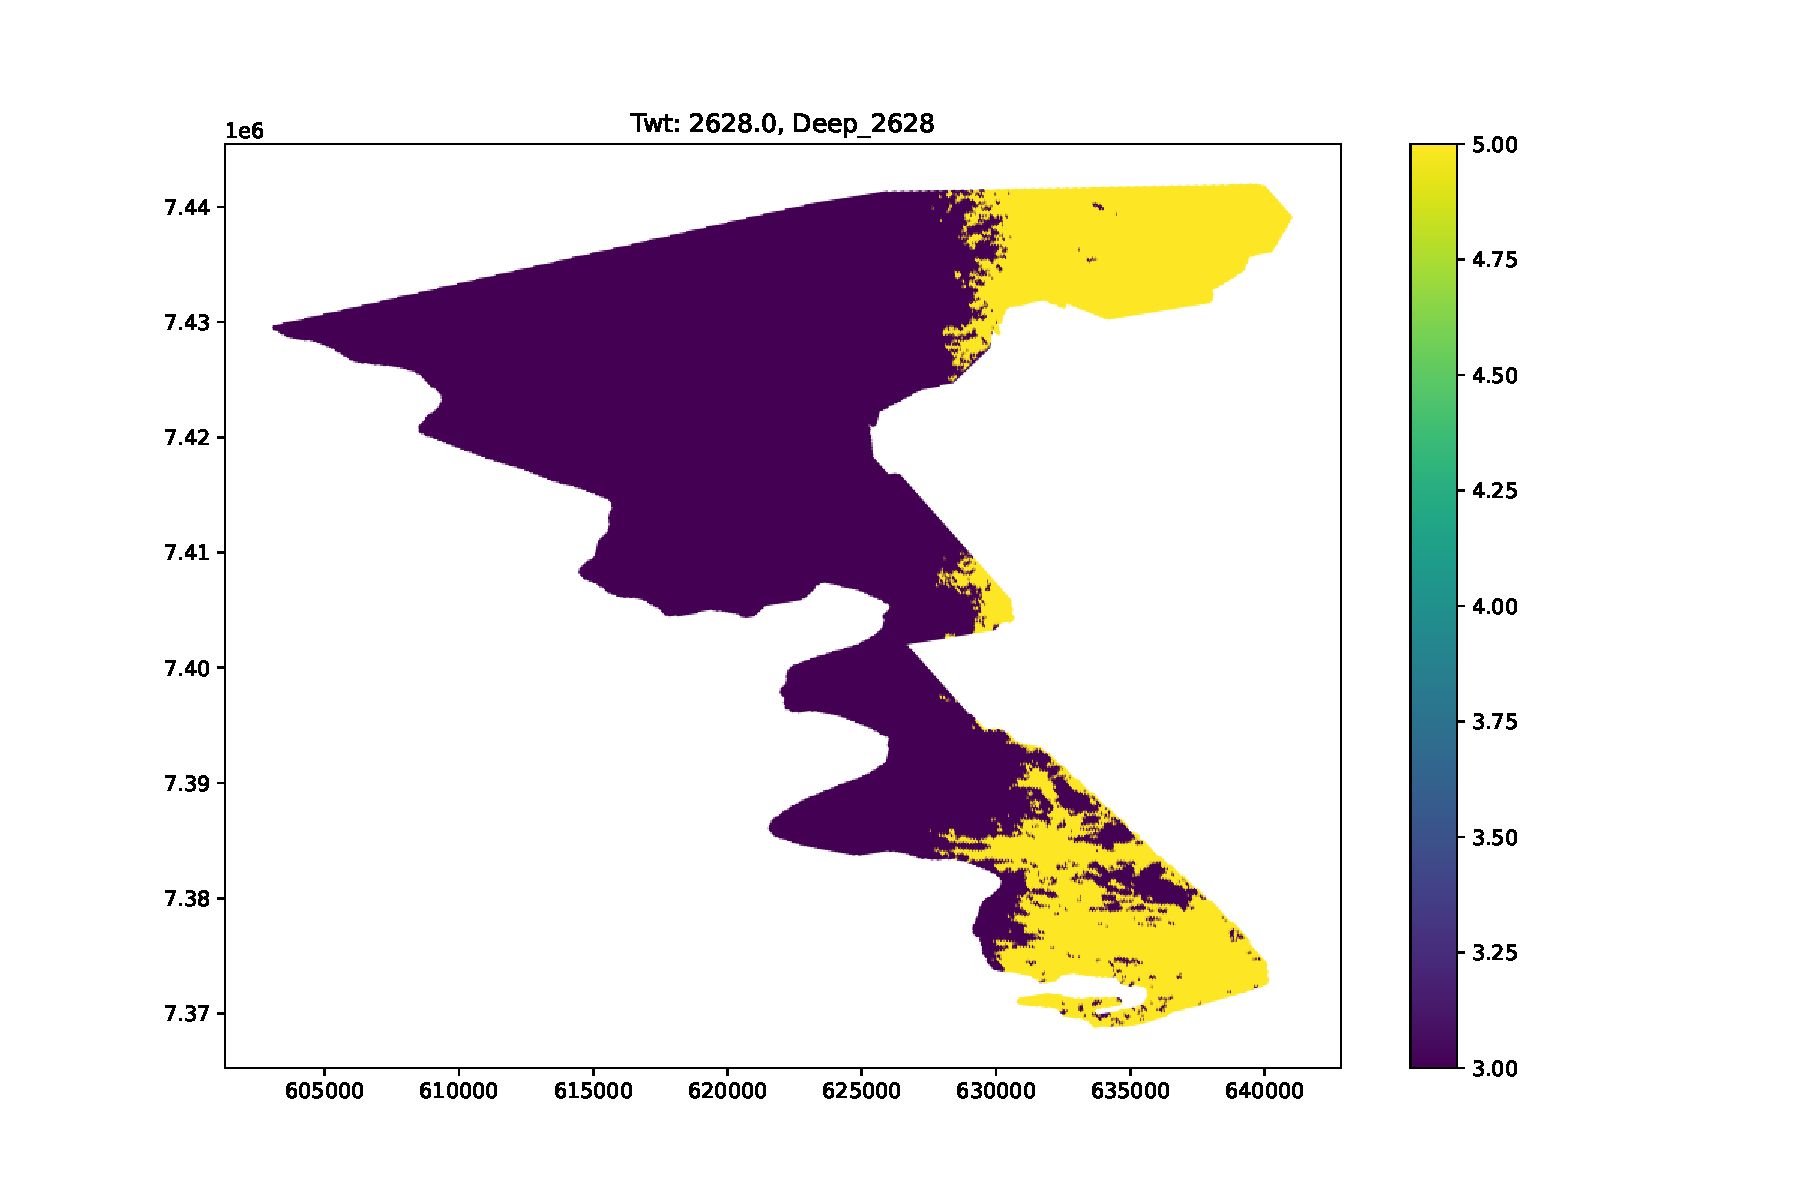
\includegraphics[width=\linewidth]{figs/cross_deep_iter6.pdf}
  \caption{Deep section}
\end{subfigure}
\caption{Representative cross-sections from iteration 6 (best ARI).}
\label{fig:cross}
\end{figure}

\section{Results}
\subsection{Intermediate Baselines}
\begin{table}[t]
\centering
\caption{Intermediate results for alternative approaches (surface ARI) and comparison with our method.}
\label{tab:baselines}
\begin{tabular}{l l l}
\toprule
\textbf{Algorithm} & \textbf{Features} & \textbf{ARI} \\
\midrule
VAE & TWT, dip illumination, consistent dip & 0.853 \\
VAE & TWT, azim cos/sin, illumination, consistent dip & 0.676 \\
VAE & TWT, azim cos/sin, dip illumination & 0.423 \\
\midrule
GMM & TWT, dip illumination, consistent dip & 0.435 \\
GMM & TWT, azim cos/sin, illumination, consistent dip & 0.374 \\
GMM & TWT, azim cos/sin, dip illumination & 0.376 \\
\midrule
Ours (Flash-KMeans + Torque) & cdp\_x, TWT, 2019\_30Hz, FF, offset\_2500 & \textbf{0.8646} \\
\bottomrule
\end{tabular}
\end{table}

\subsection{Best Configurations}
\begin{table}[t]
\centering
\caption{Best configurations (from Optuna logs).}
\label{tab:best}
\begin{tabular}{l l}
\toprule
\textbf{Metric} & \textbf{Value} \\
\midrule
Best surface ARI (previous run) & \textbf{0.8646} \\
Best surface ARI (current run)  & 0.8514 \\
\midrule
Best features (prev) & \texttt{cdp\_x, twt, 2019\_30Hz, FF, offset\_2500} \\
Best features (curr) & \texttt{cdp\_x, twt, 2019\_30Hz, offset\_ENV2500, dip\_usual} \\
\midrule
Best torque params (prev) & $k=8$, $n_n=10$, $\gamma=0.286$, $\lambda=1.025$ \\
Best torque params (curr) & $k=64$, $n_n=12$, $\gamma=0.202$, $\lambda=0.541$ \\
\bottomrule
\end{tabular}
\end{table}

\subsection{Iteration-Wise ARI}
Best previous run ARI over iterations:
\[
\{0: 0.488, 1: 0.565, 2: 0.757, 3: 0.496, 4: 0.296, 5: 0.240, 6: 0.865\}
\]
Number of feature permutations evaluated in the constrained search: \textbf{100}. In exhaustive mode up to size 7, the total is \textbf{16,383}.

\section{Discussion}
\begin{itemize}
\item High-performing feature sets consistently include \texttt{twt}, \texttt{cdp\_x}, and a mix of spectral and offset attributes.
\item Compact mixed feature sets outperform large unions.
\item Torque clustering is sensitive to $k$ and $n_{neighbors}$; low $k$ with moderate neighbors is often best.
\end{itemize}

\section{Conclusion}
We introduced a scalable two-stage clustering pipeline for seismic facies, combining Flash-KMeans compression with torque clustering on a graph of centers. Surface-projected ARI enables objective evaluation. The method scales to tens of millions of samples and yields interpretable facies partitions.

\section*{References}
\bibliographystyle{plain}
\bibliography{references}

\section*{Contribution}
\begin{itemize}
\item Student A: pipeline design, clustering experiments, metric evaluation.
\item Student B: data preprocessing, visualization, report writing.
\end{itemize}

\end{document}
